%------------------------------------------------------------------------------
\chapter{Telescope}
\label{sec:appendixTelescope}
%------------------------------------------------------------------------------

Biased residual distributions for the different telescope planes are
shown here. The biased residual on each telescope plane is defined as
the difference between the measured hit and the fitted track
position. A cut is applied to discard the tracks with $\chi^2$/NDF
higher than 100.


\begin{figure}[htbp] \centering
  \begin{subfigure}[b]{0.3\textwidth}
    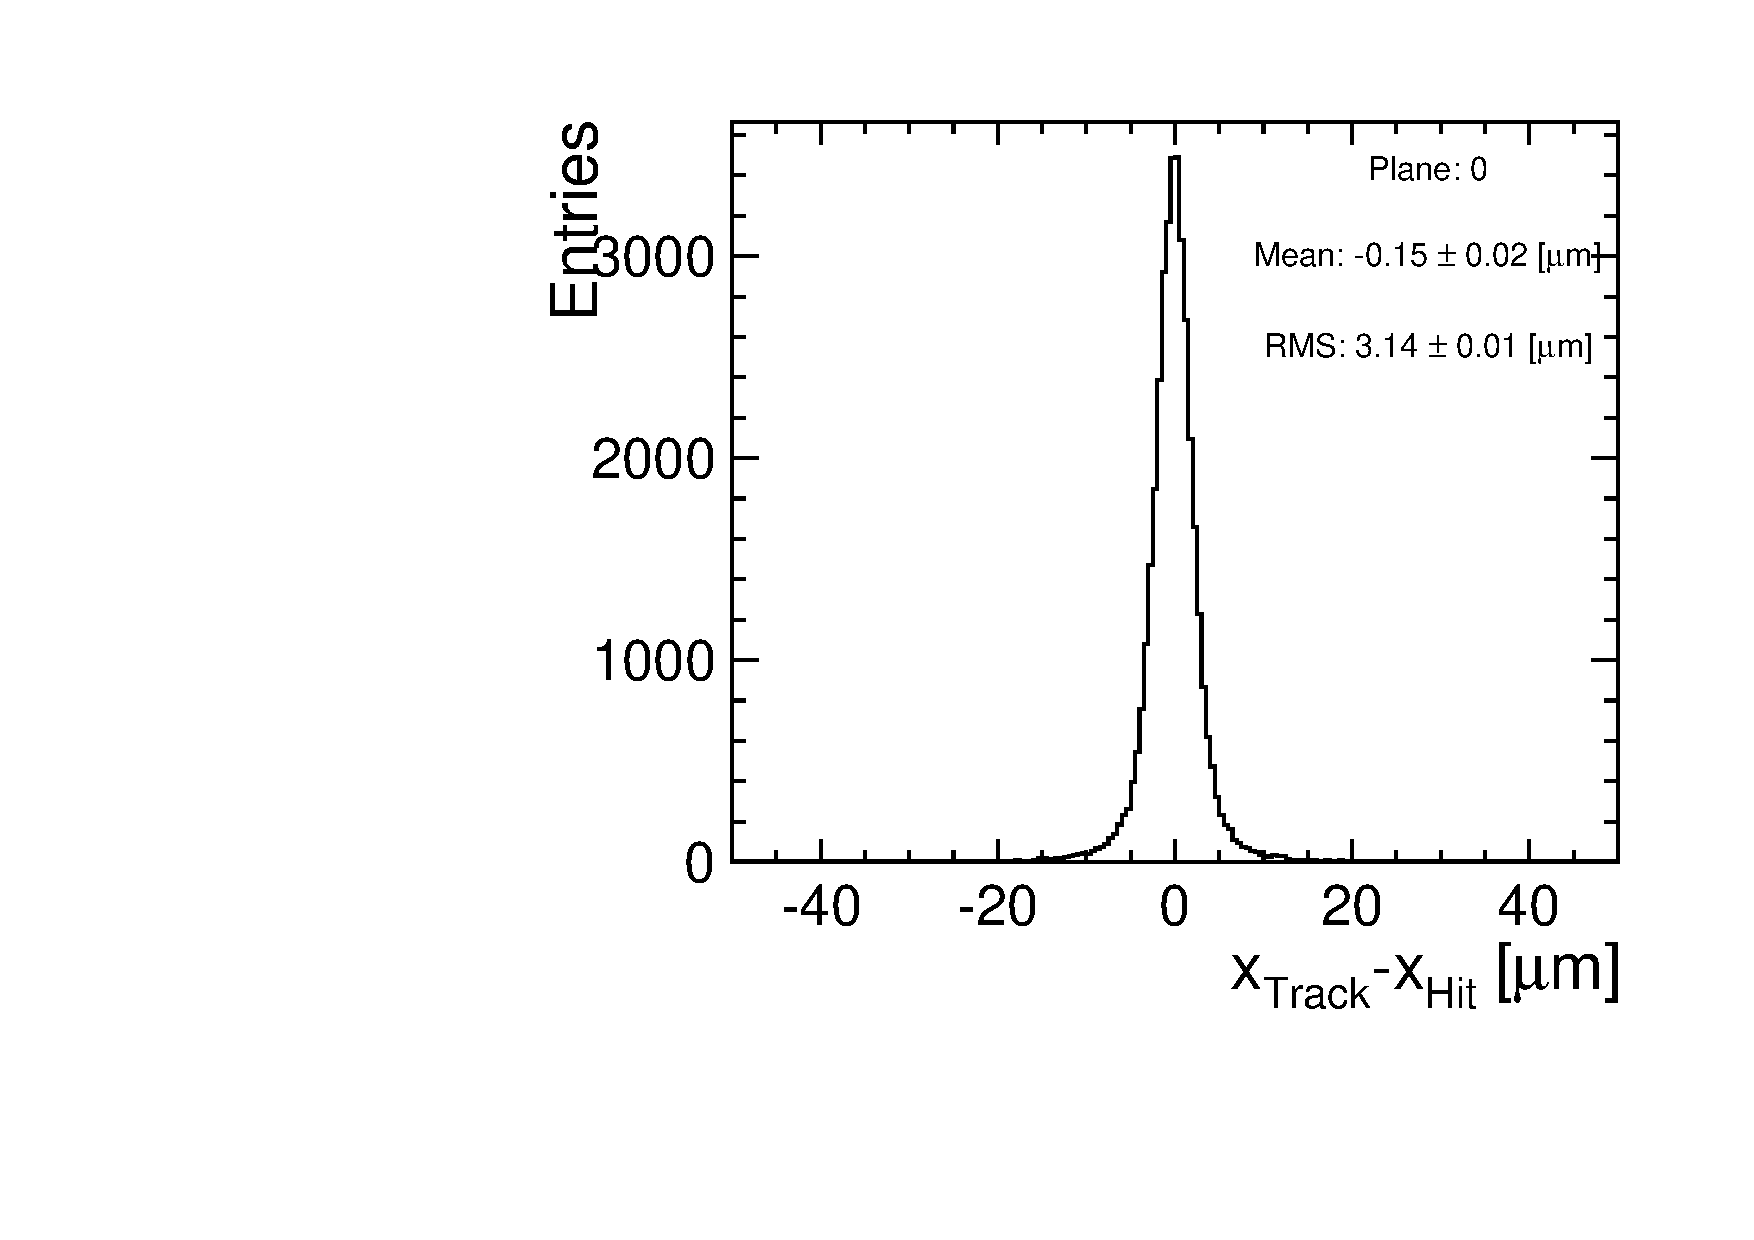
\includegraphics[width=\textwidth]{figures/Telescope/biasedResiduals/BiasedResiduals_run661_PlaneXRMS0.pdf}
    \caption{Telescope plane 0}
  \end{subfigure}\hfill
  \begin{subfigure}[b]{0.3\textwidth}
    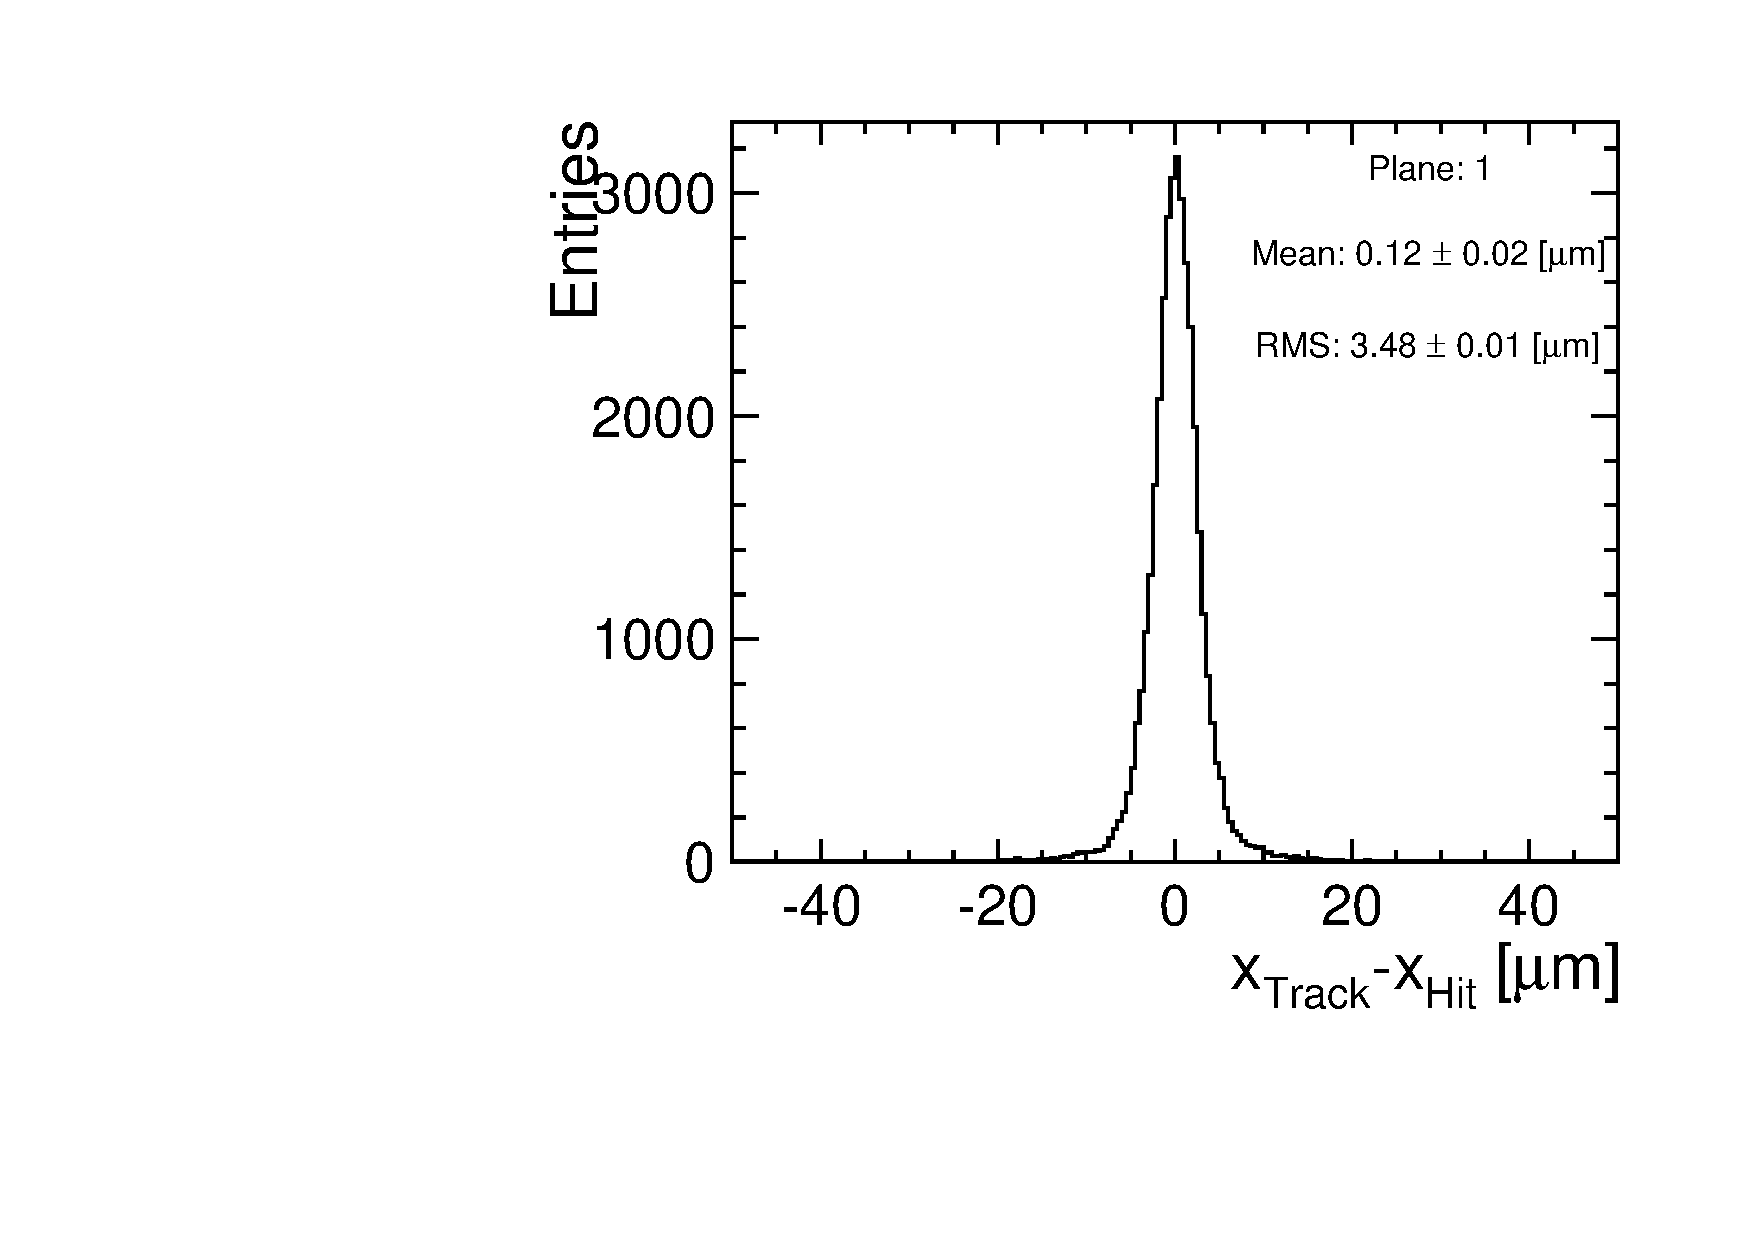
\includegraphics[width=\textwidth]{figures/Telescope/biasedResiduals/BiasedResiduals_run661_PlaneXRMS1.pdf}
    \caption{Telescope plane 1}
  \end{subfigure}\hfill
  \begin{subfigure}[b]{0.3\textwidth}
    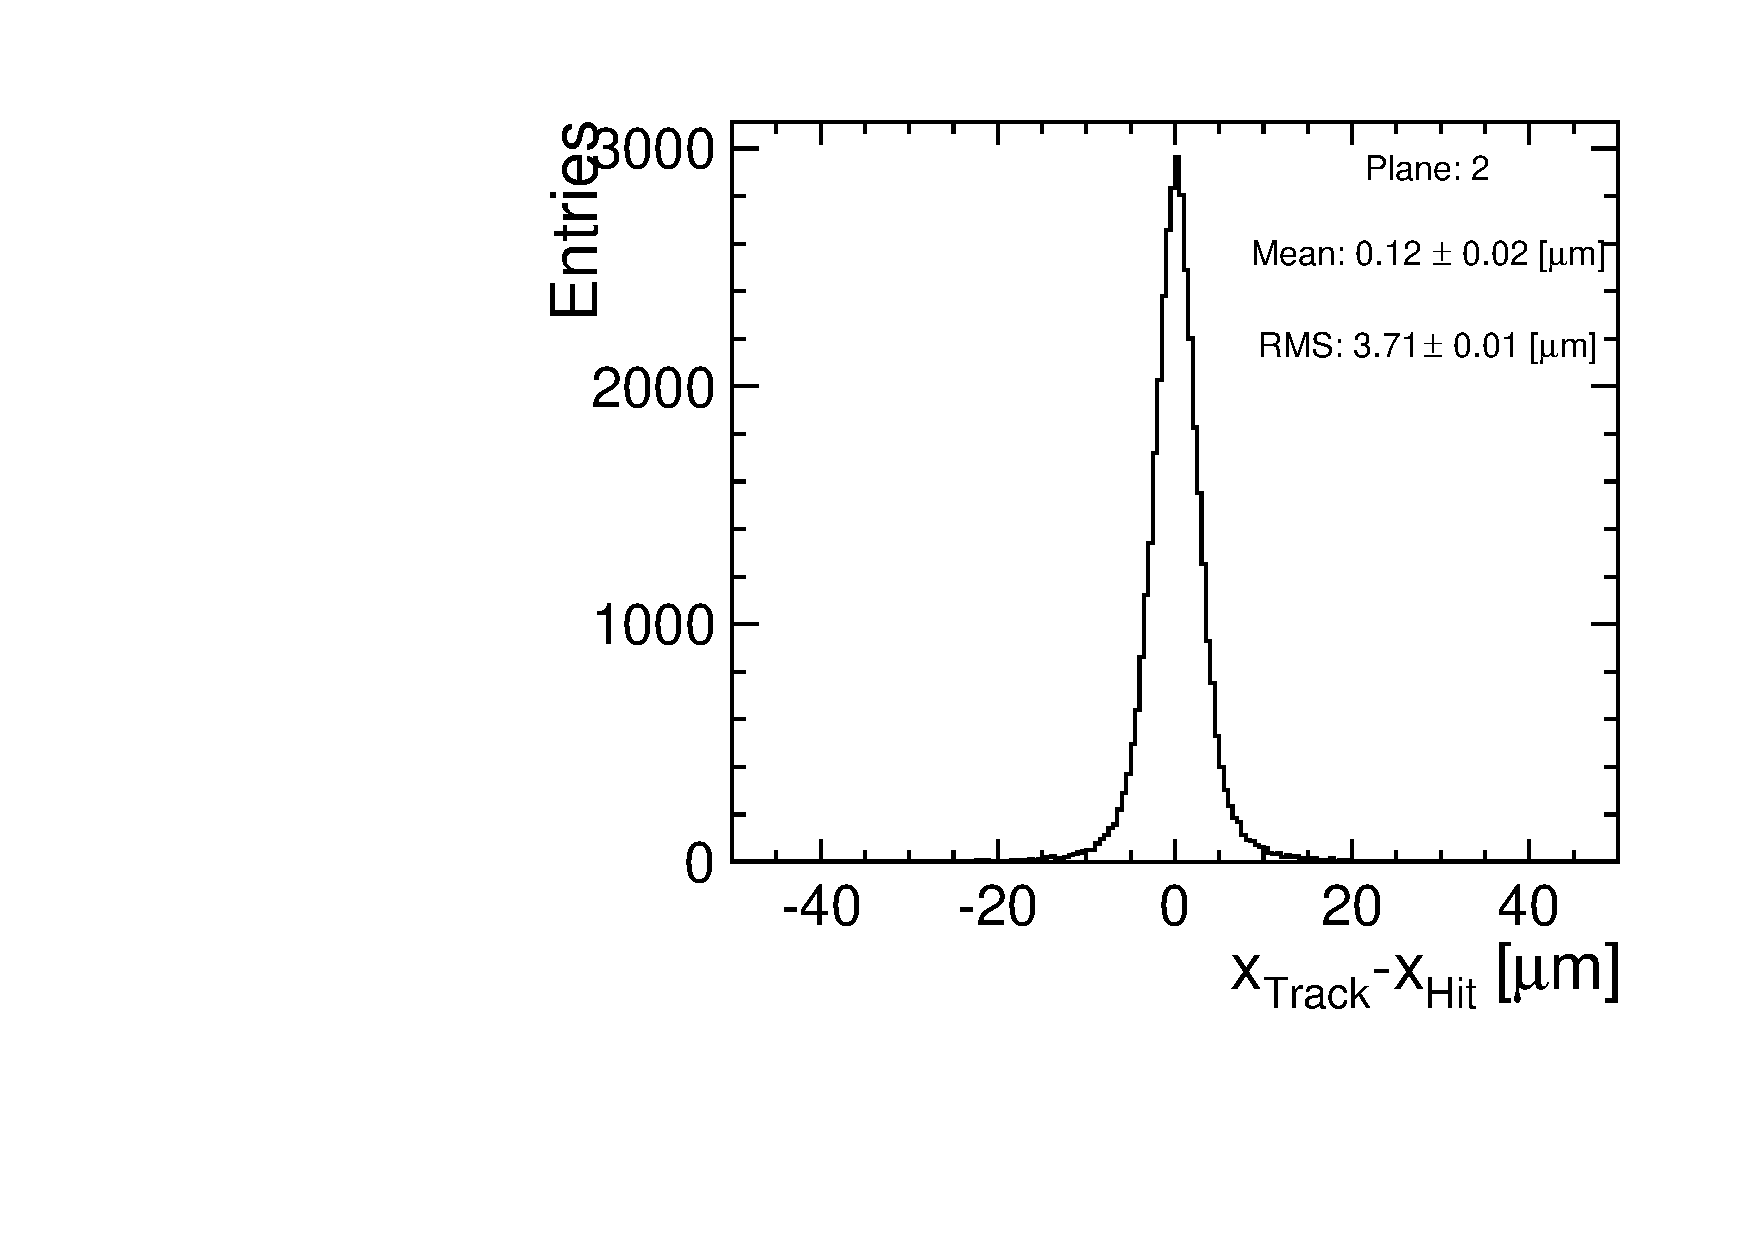
\includegraphics[width=\textwidth]{figures/Telescope/biasedResiduals/BiasedResiduals_run661_PlaneXRMS2.pdf}
    \caption{Telescope plane 2}
  \end{subfigure} \\
  \begin{subfigure}[b]{0.3\textwidth}
    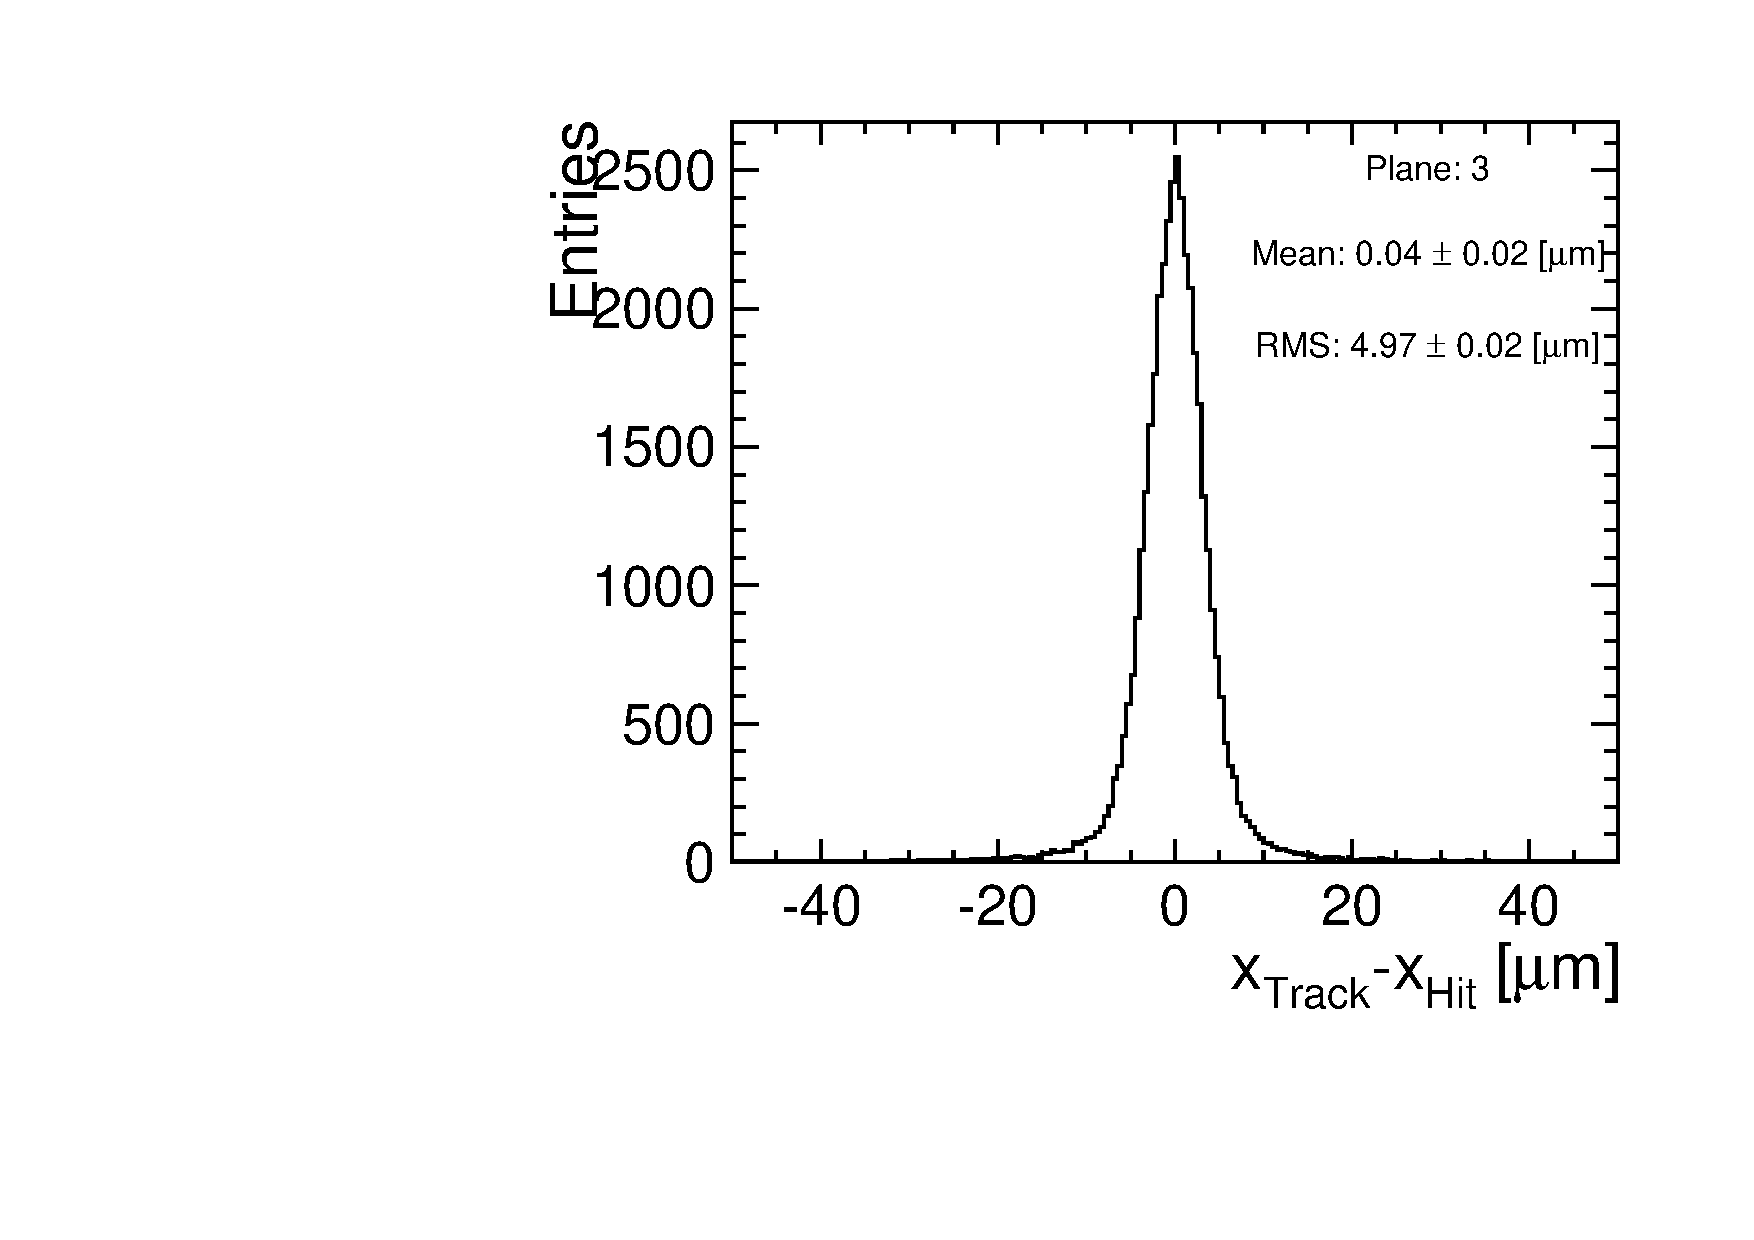
\includegraphics[width=\textwidth]{figures/Telescope/biasedResiduals/BiasedResiduals_run661_PlaneXRMS3.pdf}
    \caption{Telescope plane 3}
  \end{subfigure}\hfill
  \begin{subfigure}[b]{0.3\textwidth}
    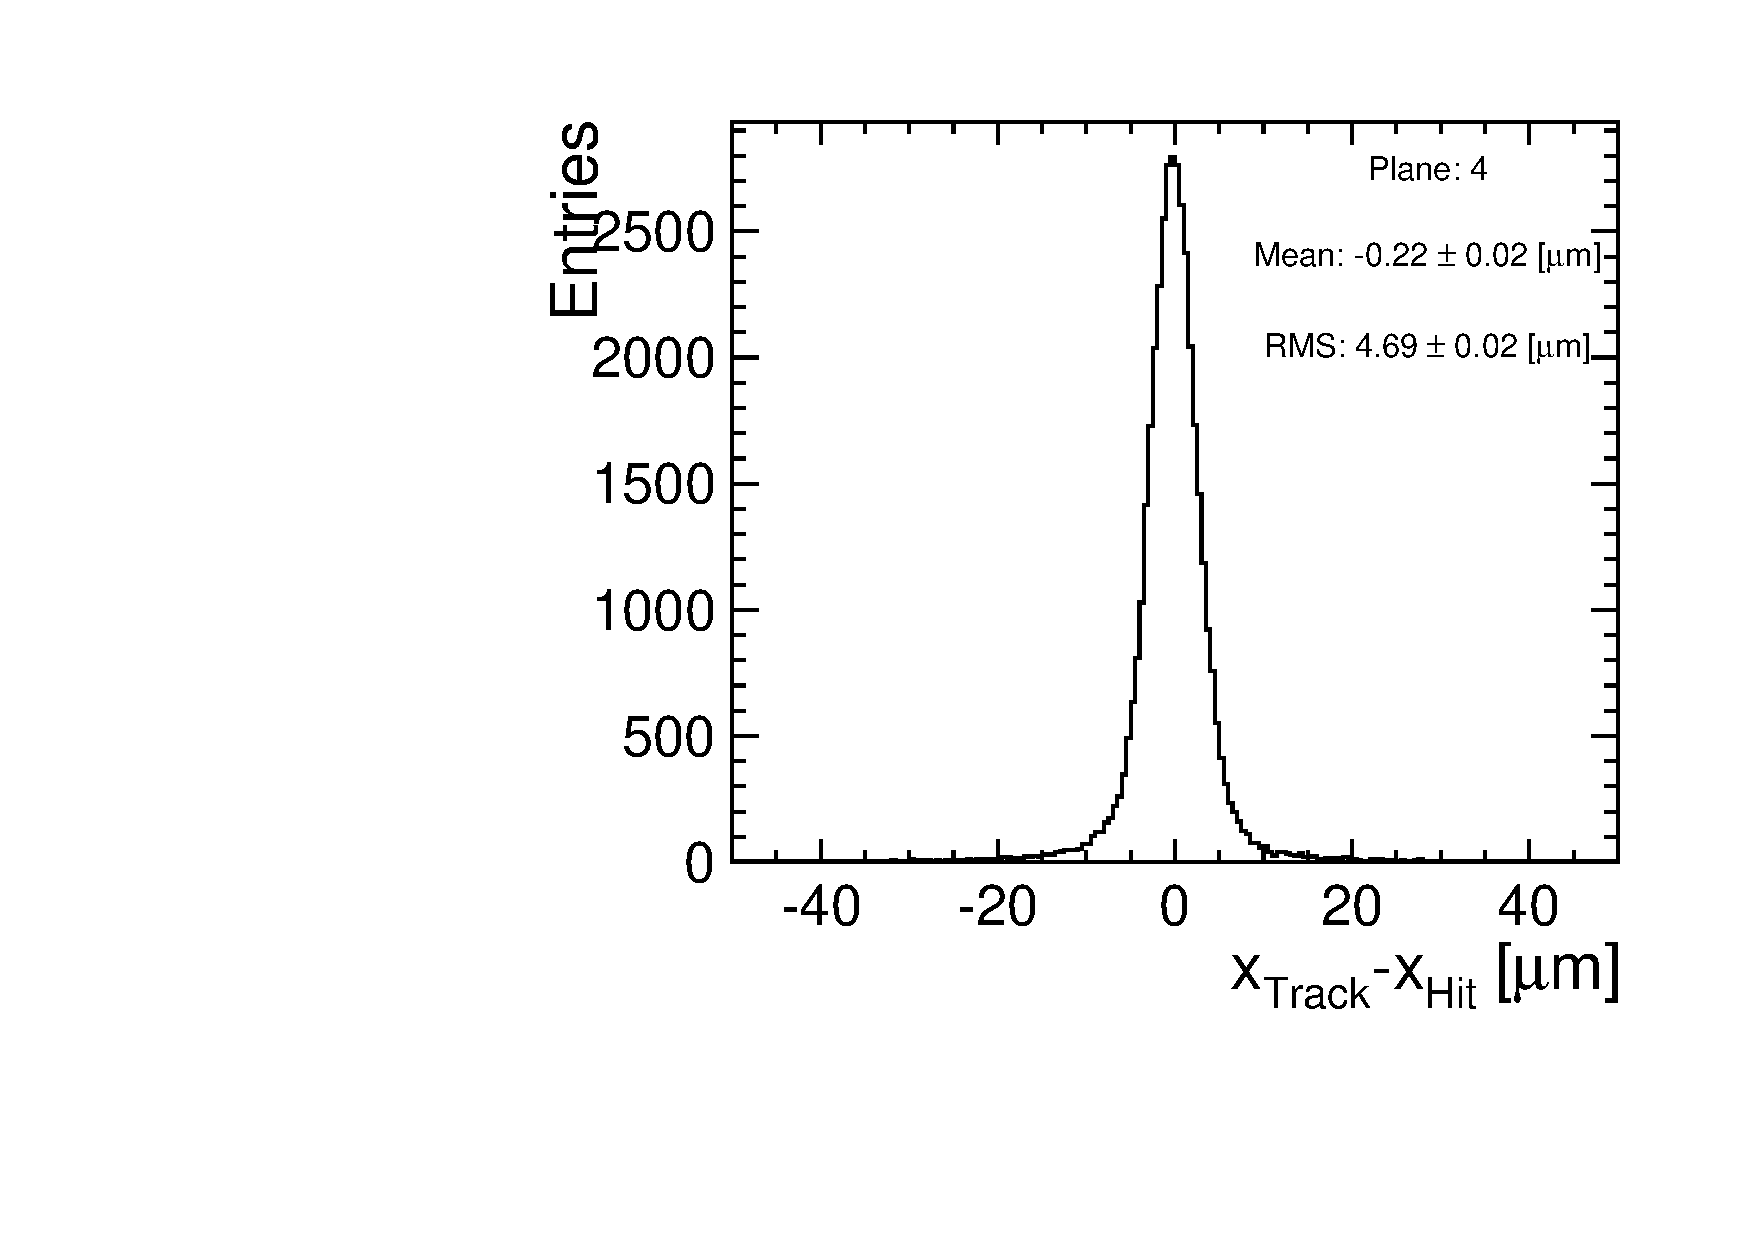
\includegraphics[width=\textwidth]{figures/Telescope/biasedResiduals/BiasedResiduals_run661_PlaneXRMS4.pdf}
    \caption{Telescope plane 4}
  \end{subfigure}\hfill
  \begin{subfigure}[b]{0.3\textwidth}
    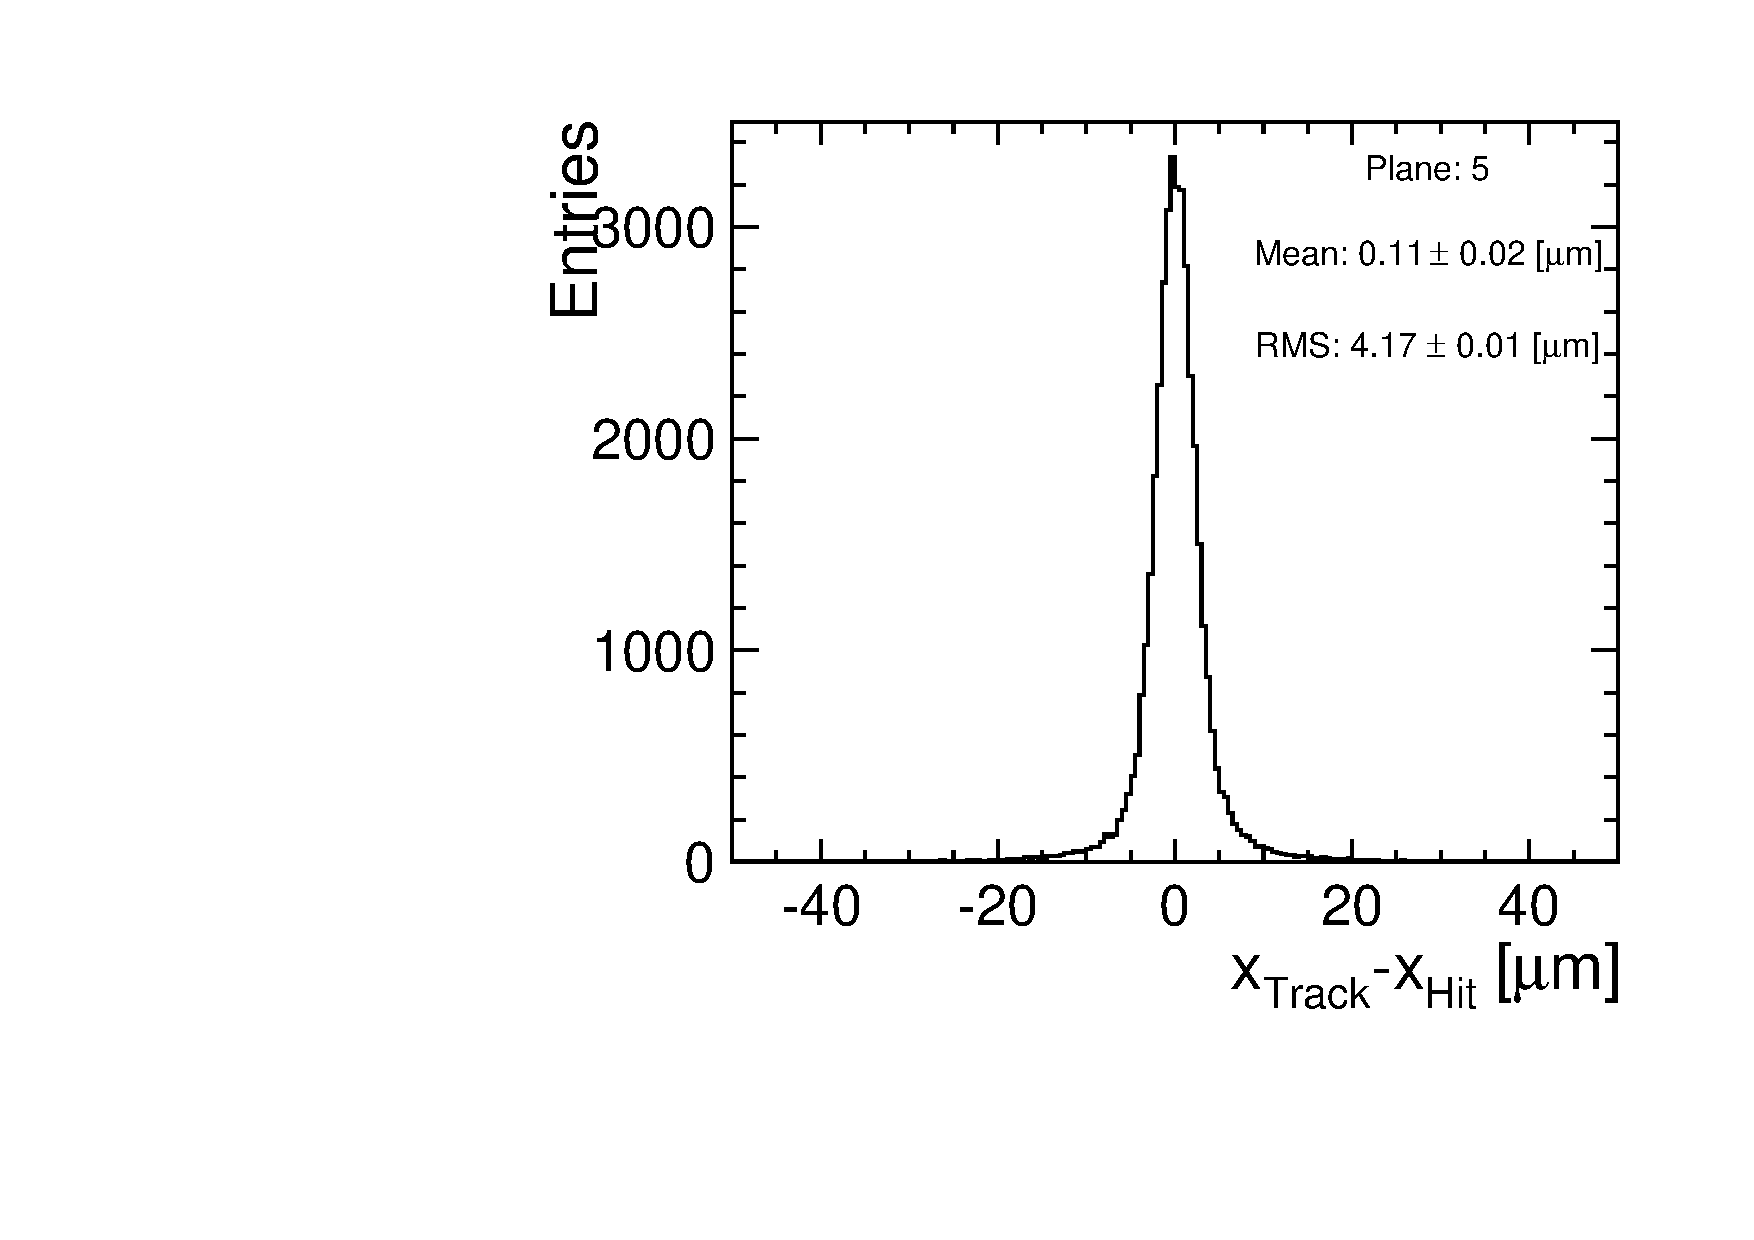
\includegraphics[width=\textwidth]{figures/Telescope/biasedResiduals/BiasedResiduals_run661_PlaneXRMS5.pdf}
    \caption{Telescope plane 5}
  \end{subfigure}
  \caption{Biased residual distribution in x-direction obtained in
    data for each telescope plane. The RMS of the residual is also
    shown.}
  \label{fig:telescope_biasedResiduals_data_X}
\end{figure}

\begin{figure}[htbp] \centering
  \begin{subfigure}[b]{0.3\textwidth}
    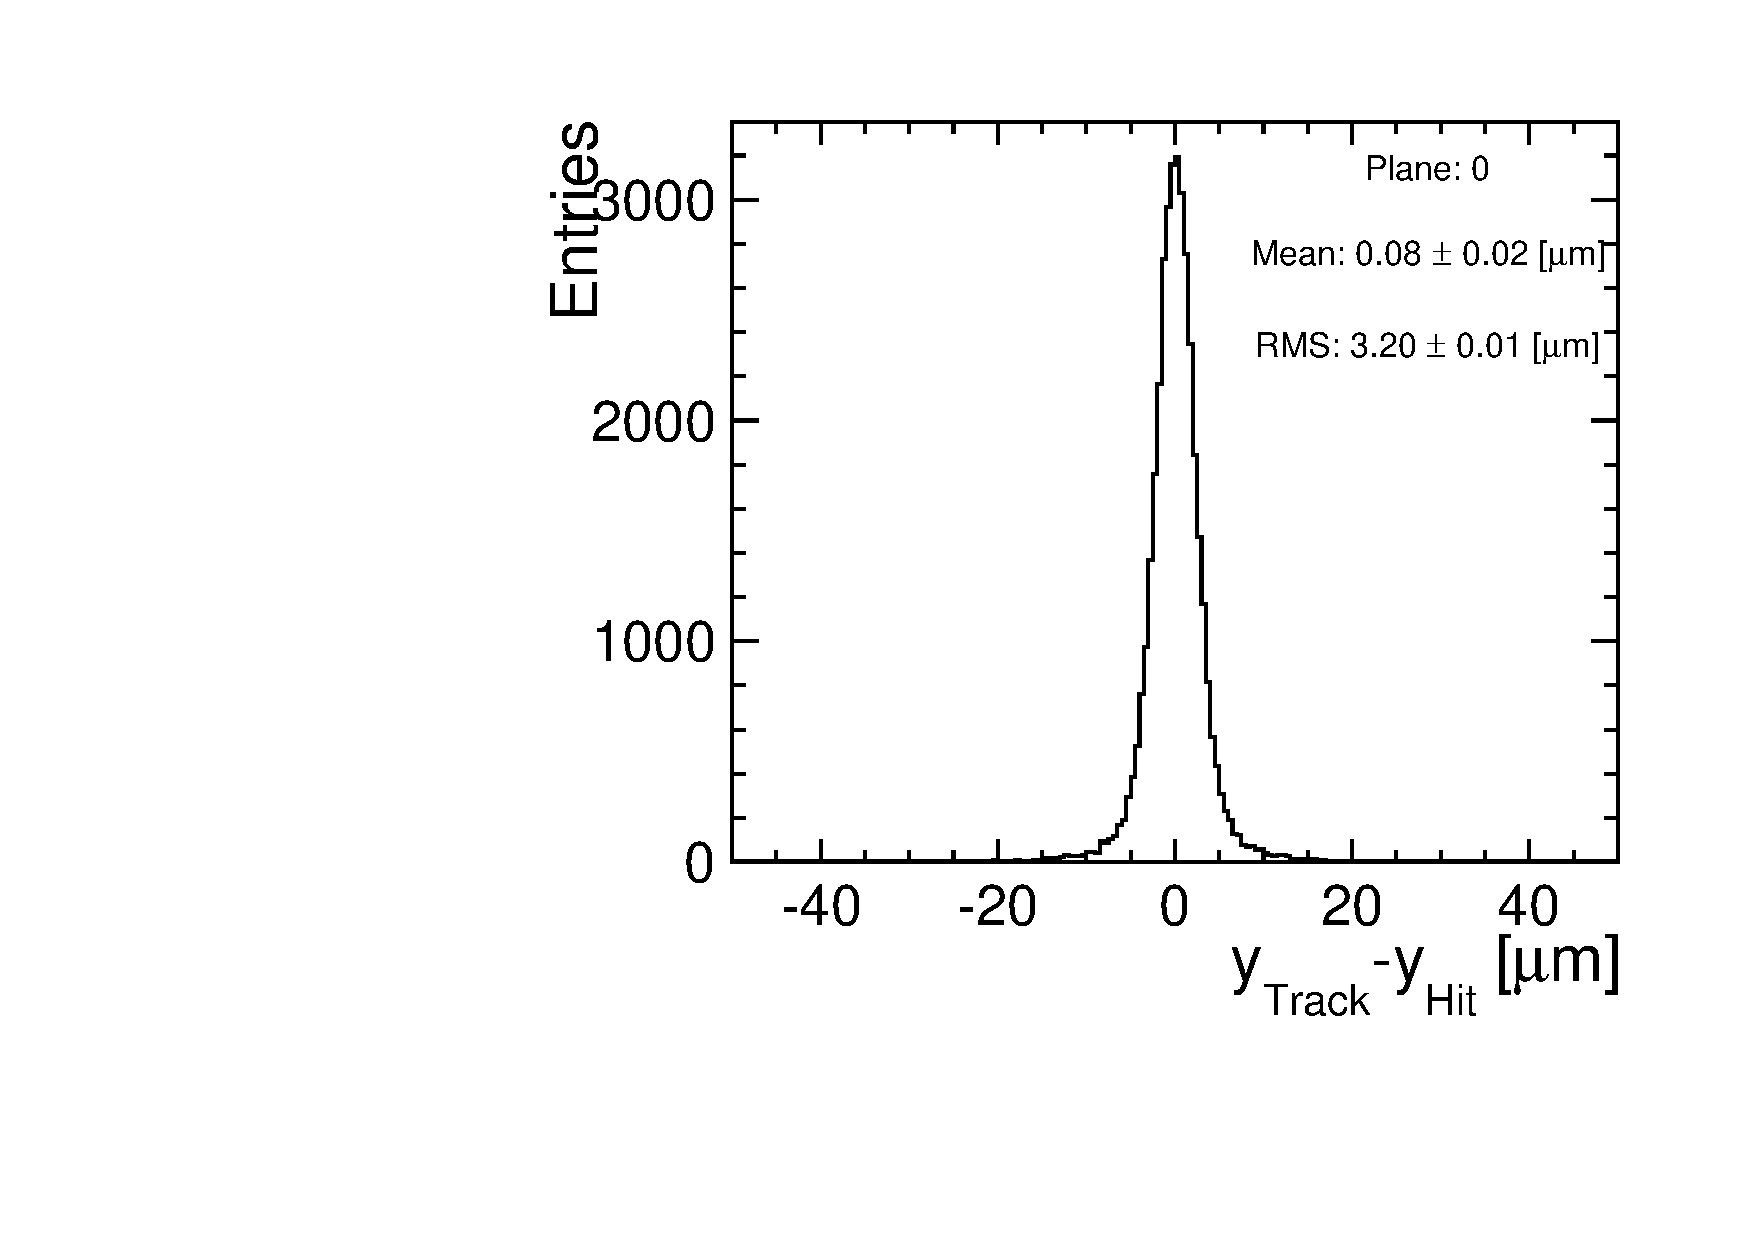
\includegraphics[width=\textwidth]{figures/Telescope/biasedResiduals/BiasedResiduals_run661_PlaneYRMS0.pdf}
    \caption{Telescope  plane 0}
  \end{subfigure}\hfill
  \begin{subfigure}[b]{0.3\textwidth}
    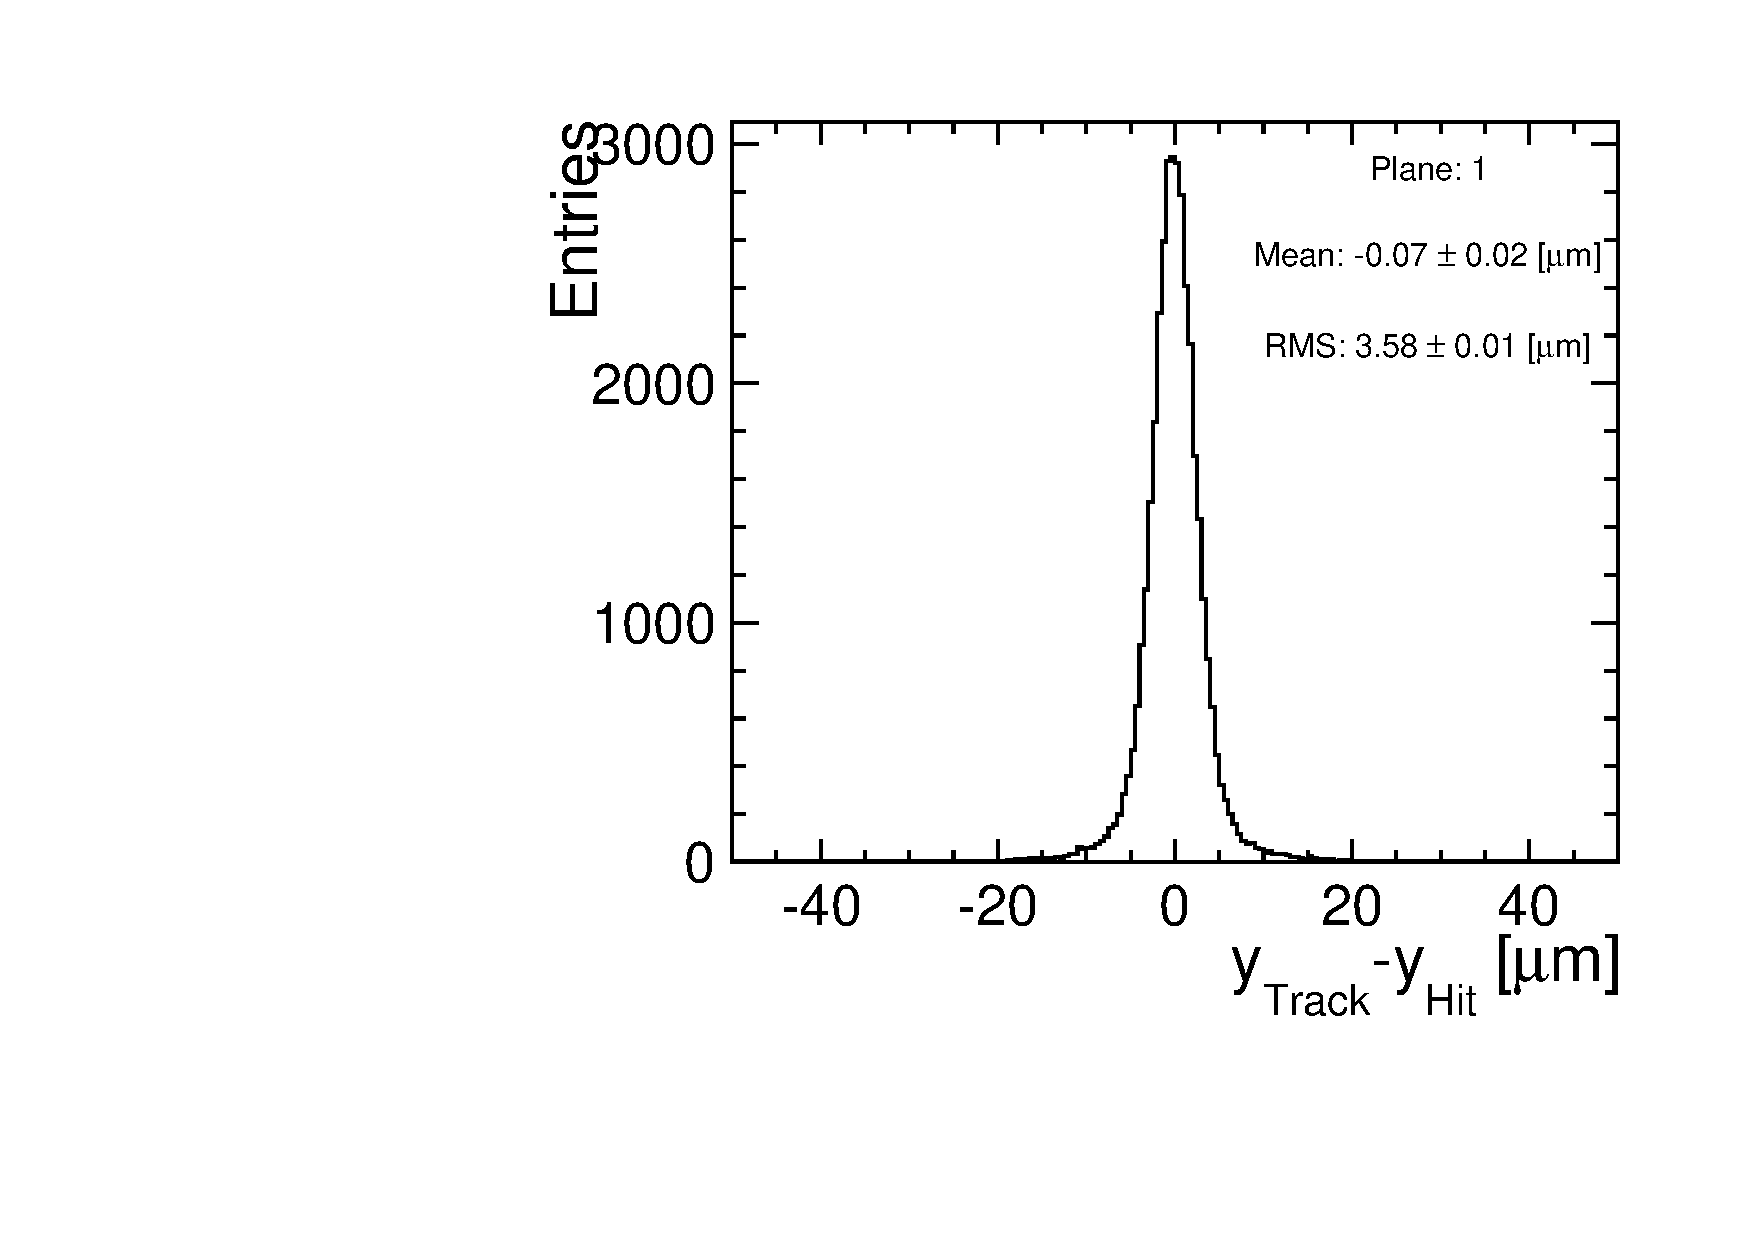
\includegraphics[width=\textwidth]{figures/Telescope/biasedResiduals/BiasedResiduals_run661_PlaneYRMS1.pdf}
    \caption{Telescope  plane 1}
  \end{subfigure}\hfill
  \begin{subfigure}[b]{0.3\textwidth}
    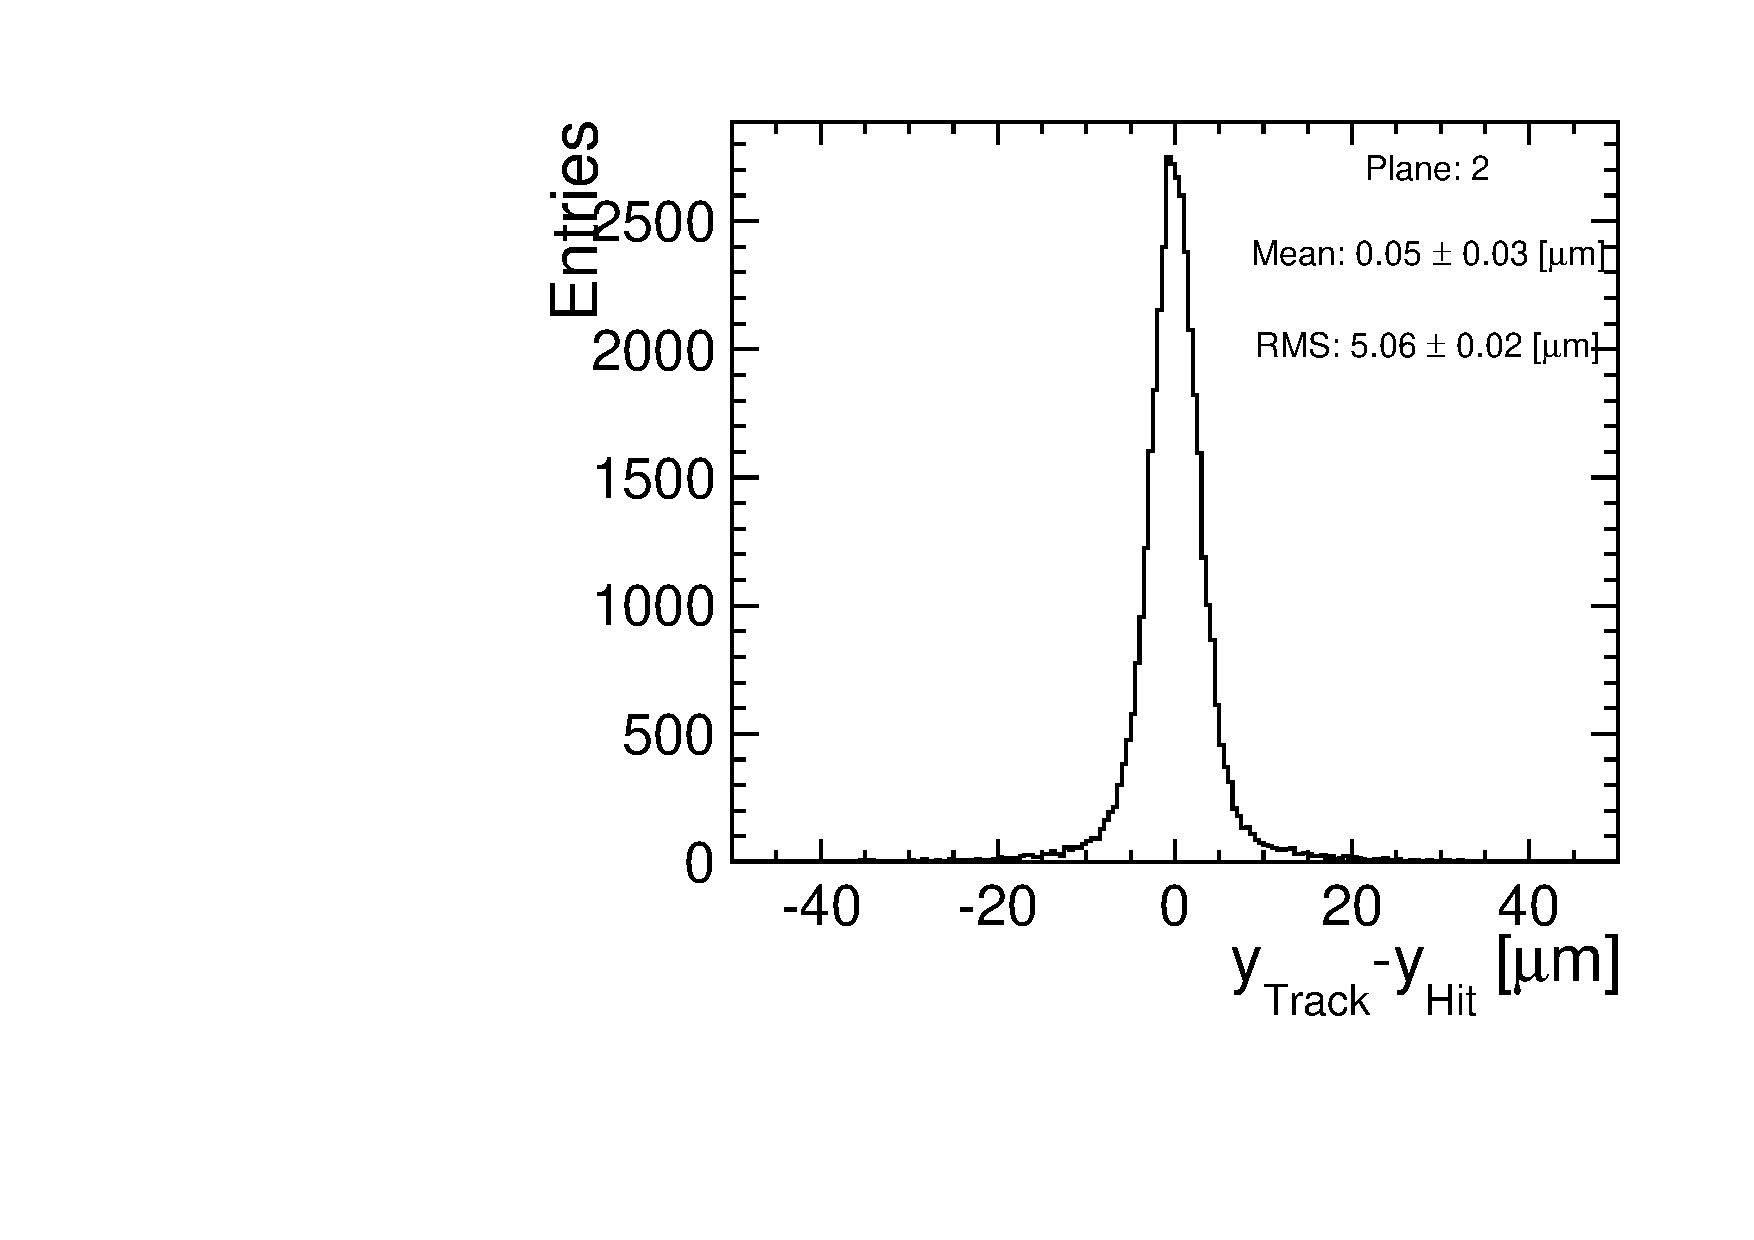
\includegraphics[width=\textwidth]{figures/Telescope/biasedResiduals/BiasedResiduals_run661_PlaneYRMS2.pdf}
    \caption{Telescope  plane 2}
  \end{subfigure} \\
  \begin{subfigure}[b]{0.3\textwidth}
    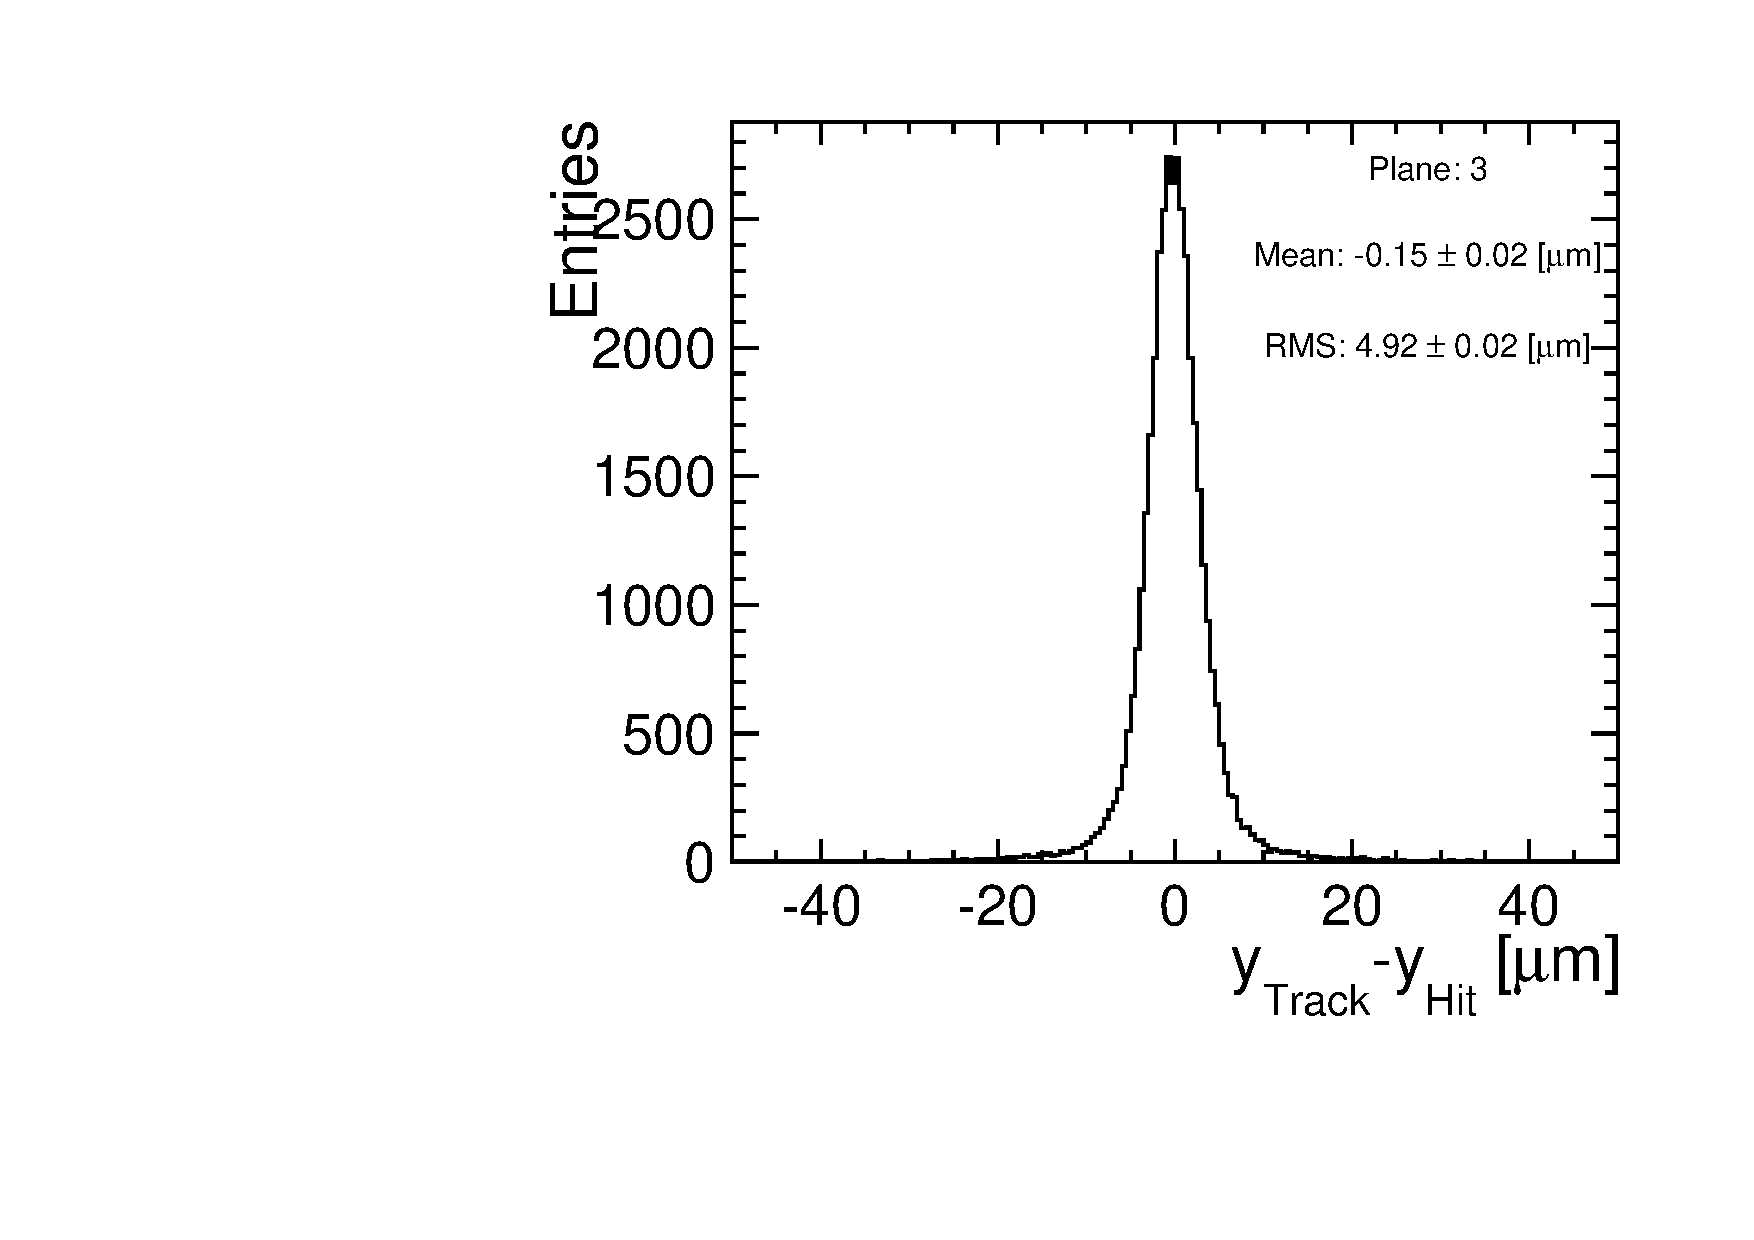
\includegraphics[width=\textwidth]{figures/Telescope/biasedResiduals/BiasedResiduals_run661_PlaneYRMS3.pdf}
    \caption{Telescope  plane 3}
  \end{subfigure}\hfill
  \begin{subfigure}[b]{0.3\textwidth}
    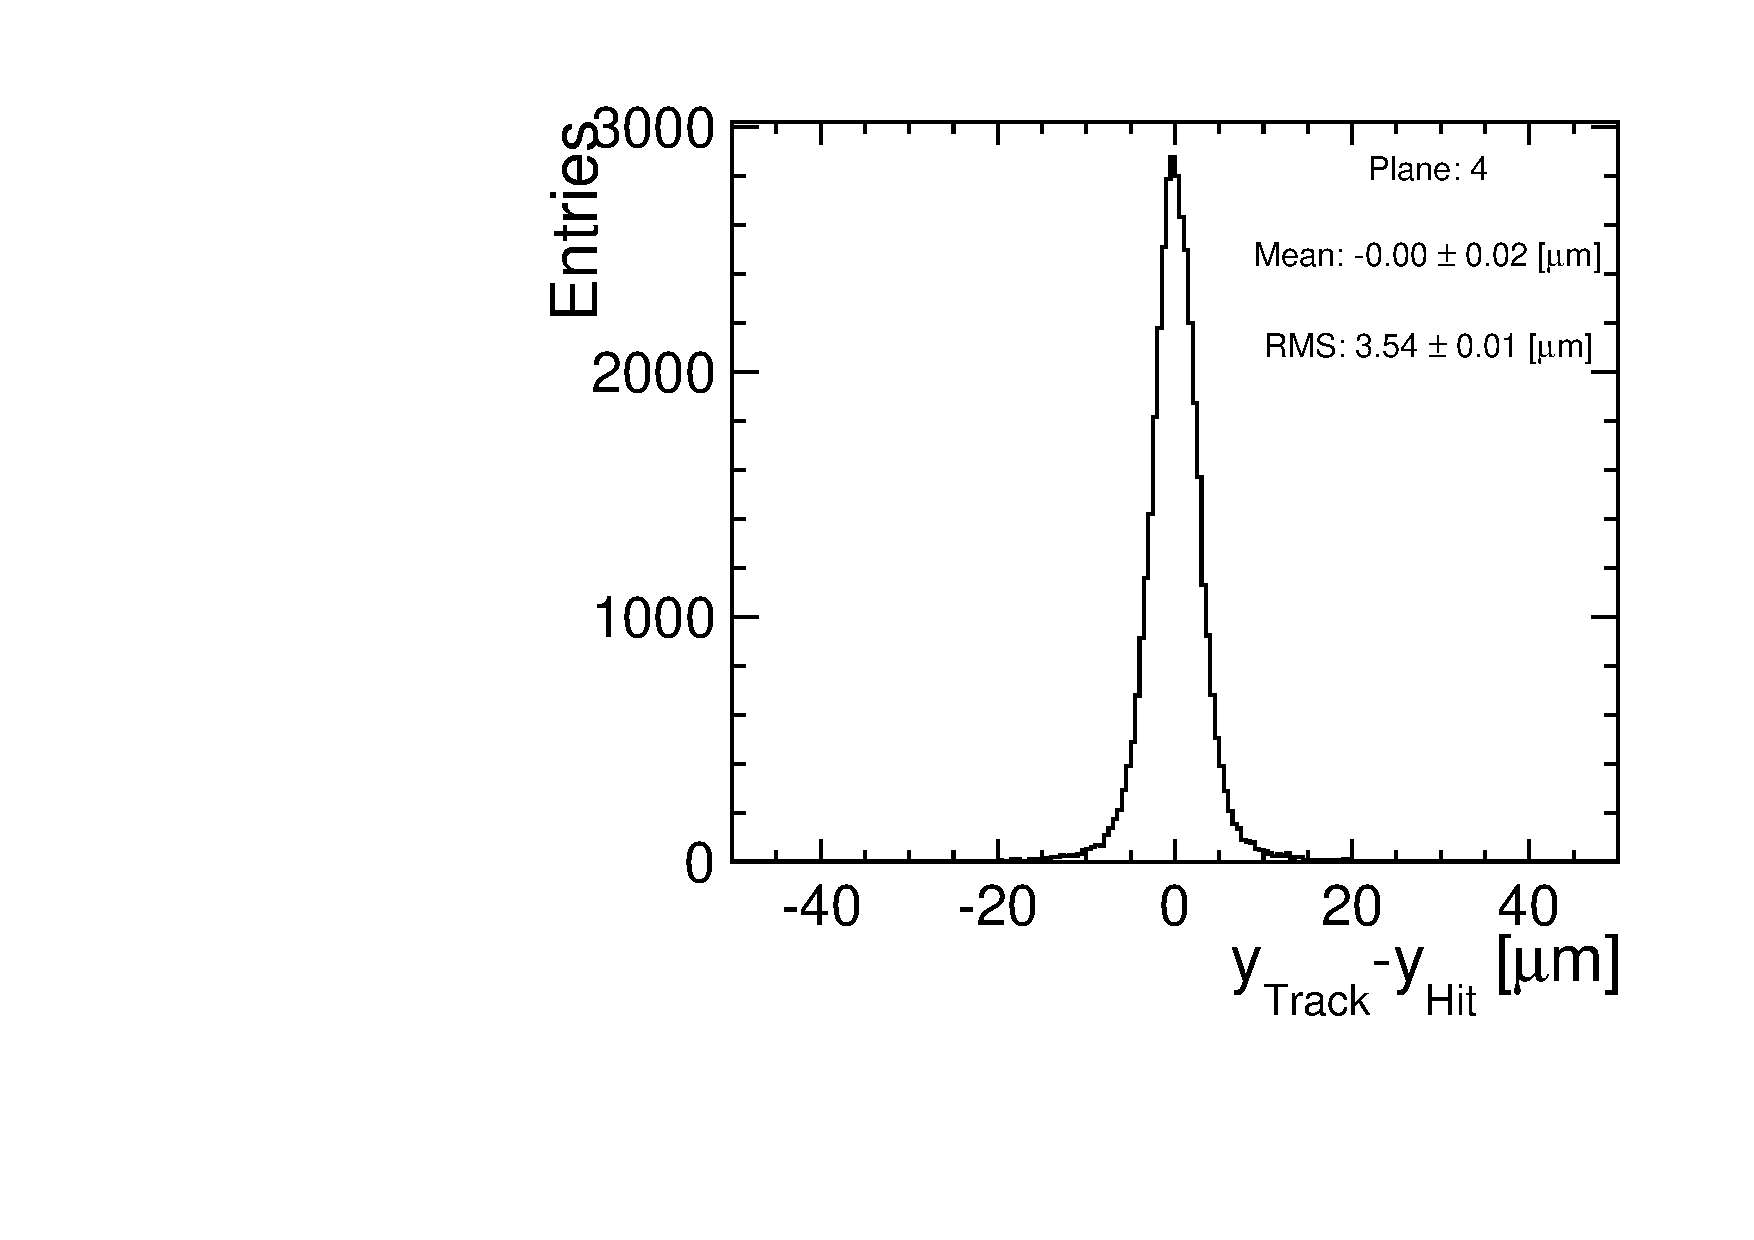
\includegraphics[width=\textwidth]{figures/Telescope/biasedResiduals/BiasedResiduals_run661_PlaneYRMS4.pdf}
    \caption{Telescope  plane 4}
  \end{subfigure}\hfill
  \begin{subfigure}[b]{0.3\textwidth}
    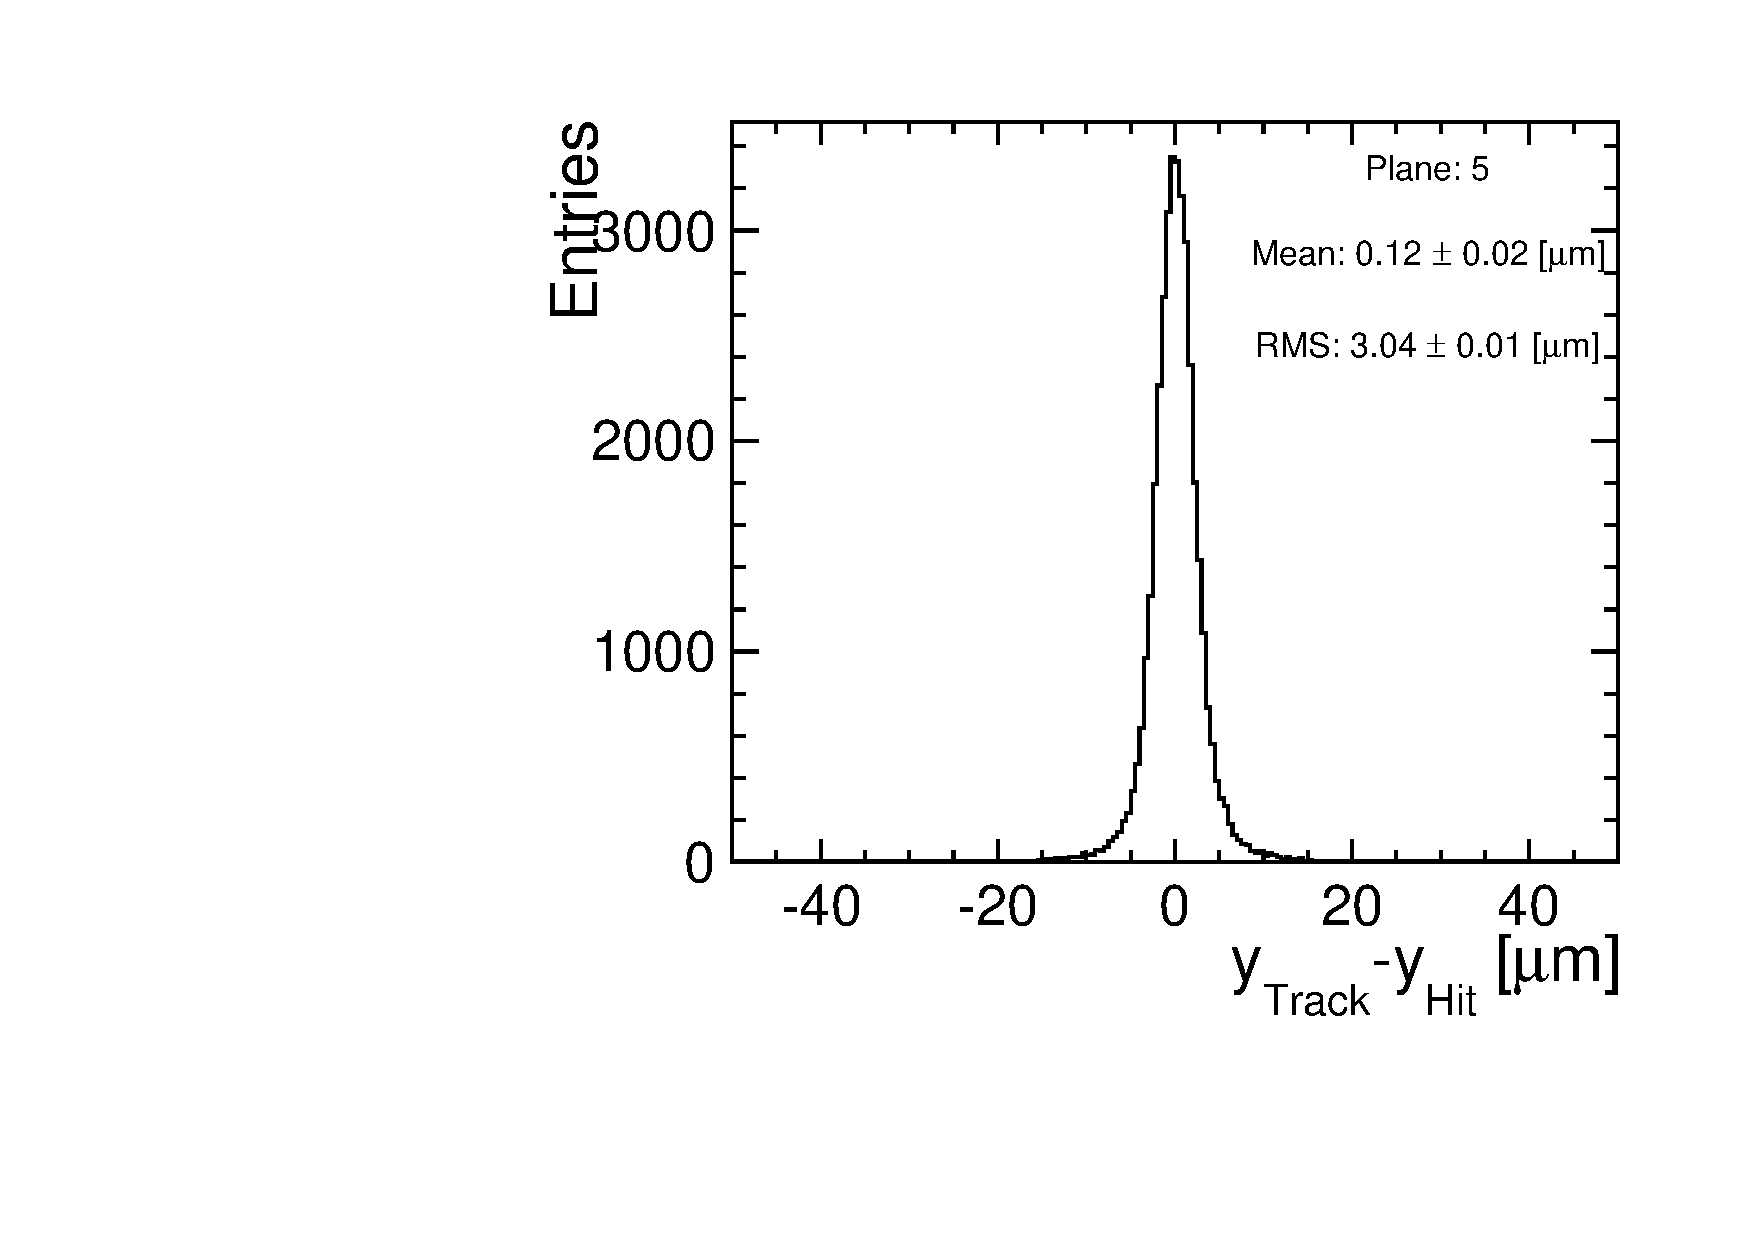
\includegraphics[width=\textwidth]{figures/Telescope/biasedResiduals/BiasedResiduals_run661_PlaneYRMS5.pdf}
    \caption{Telescope  plane 5}
  \end{subfigure}
  \caption{Biased residual distribution in y-direction obtained in
    data for each telescope plane. The RMS of the residual is also
    shown.}
  \label{fig:telescope_biasedResiduals_data_Y}
\end{figure}


\begin{figure}[htbp] \centering
  \begin{subfigure}[b]{0.3\textwidth}
    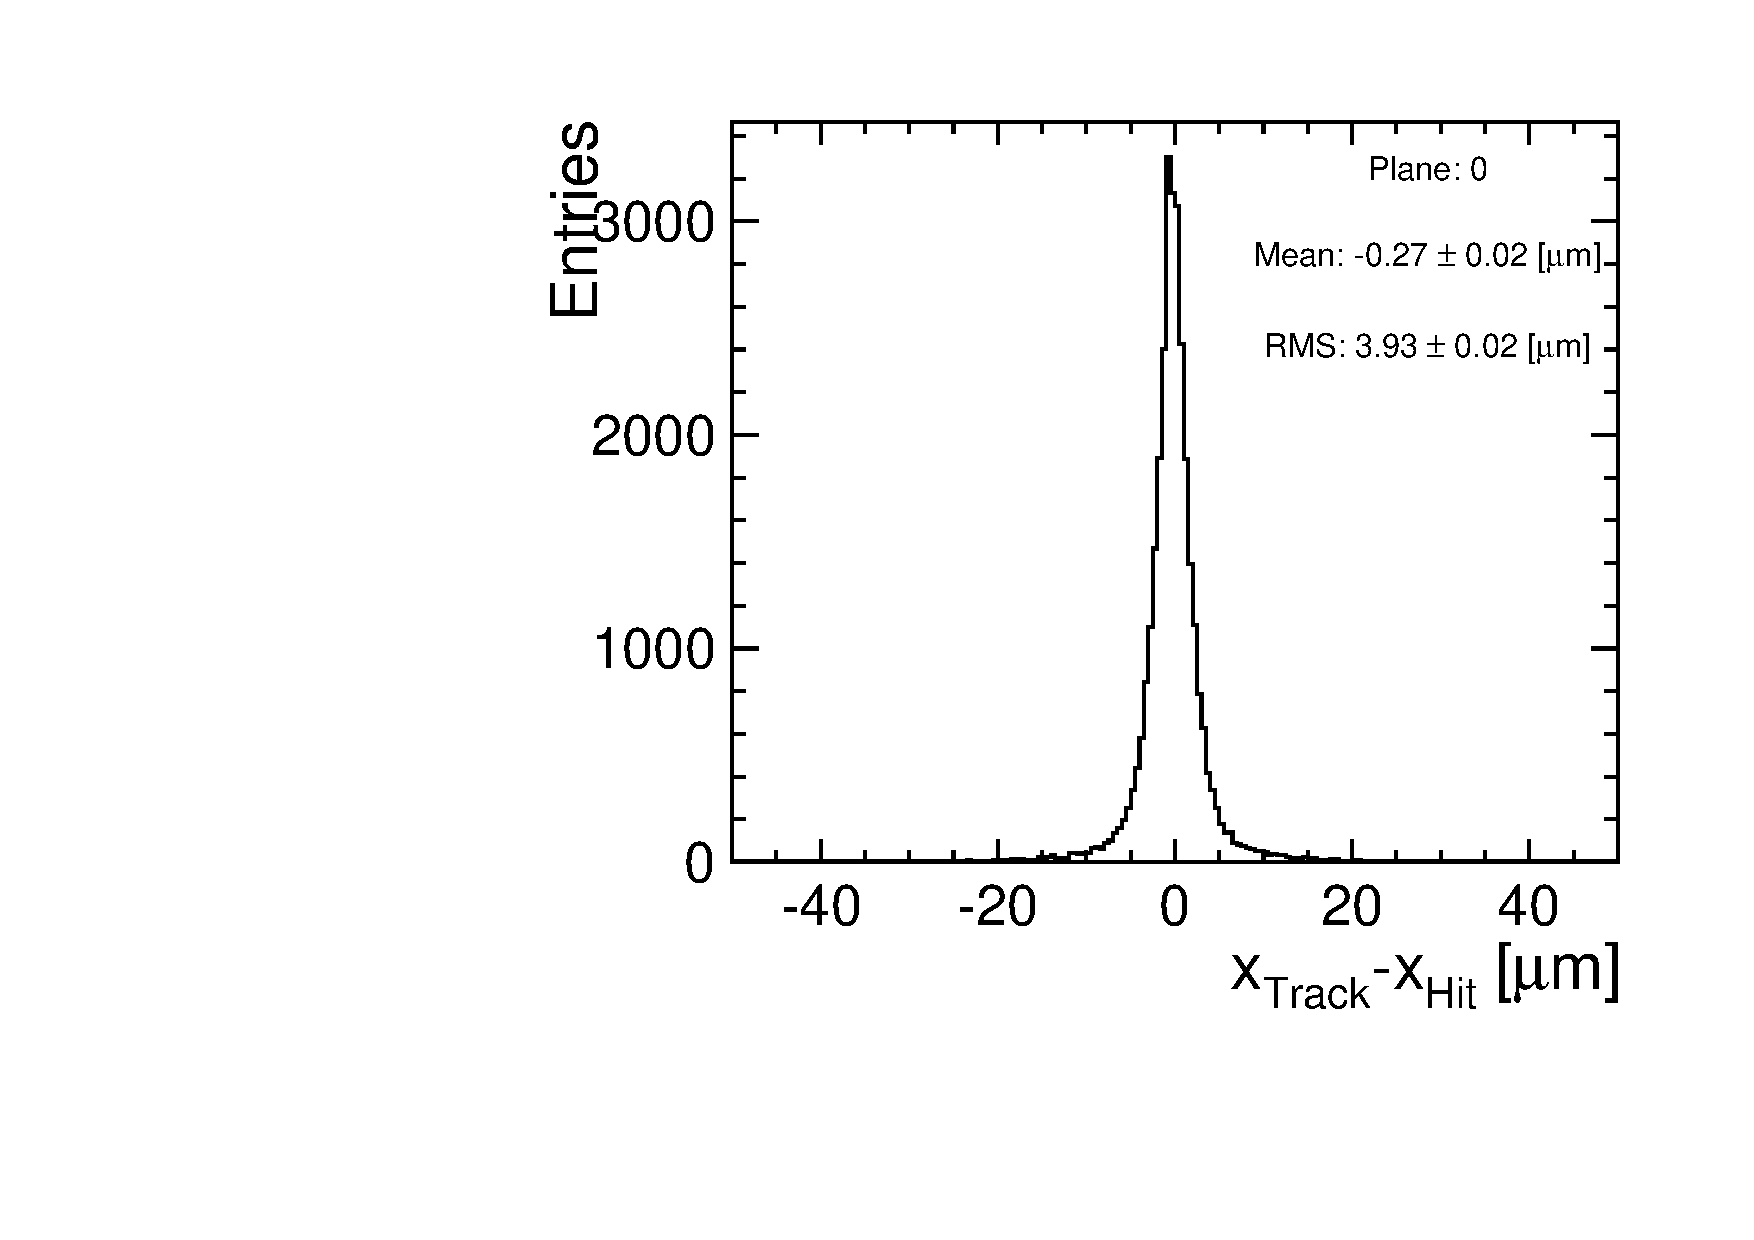
\includegraphics[width=\textwidth]{figures/Telescope/biasedResiduals/BiasedResiduals_run49_PlaneXRMS0.pdf}
    \caption{Telescope plane 0}
  \end{subfigure}\hfill
  \begin{subfigure}[b]{0.3\textwidth}
    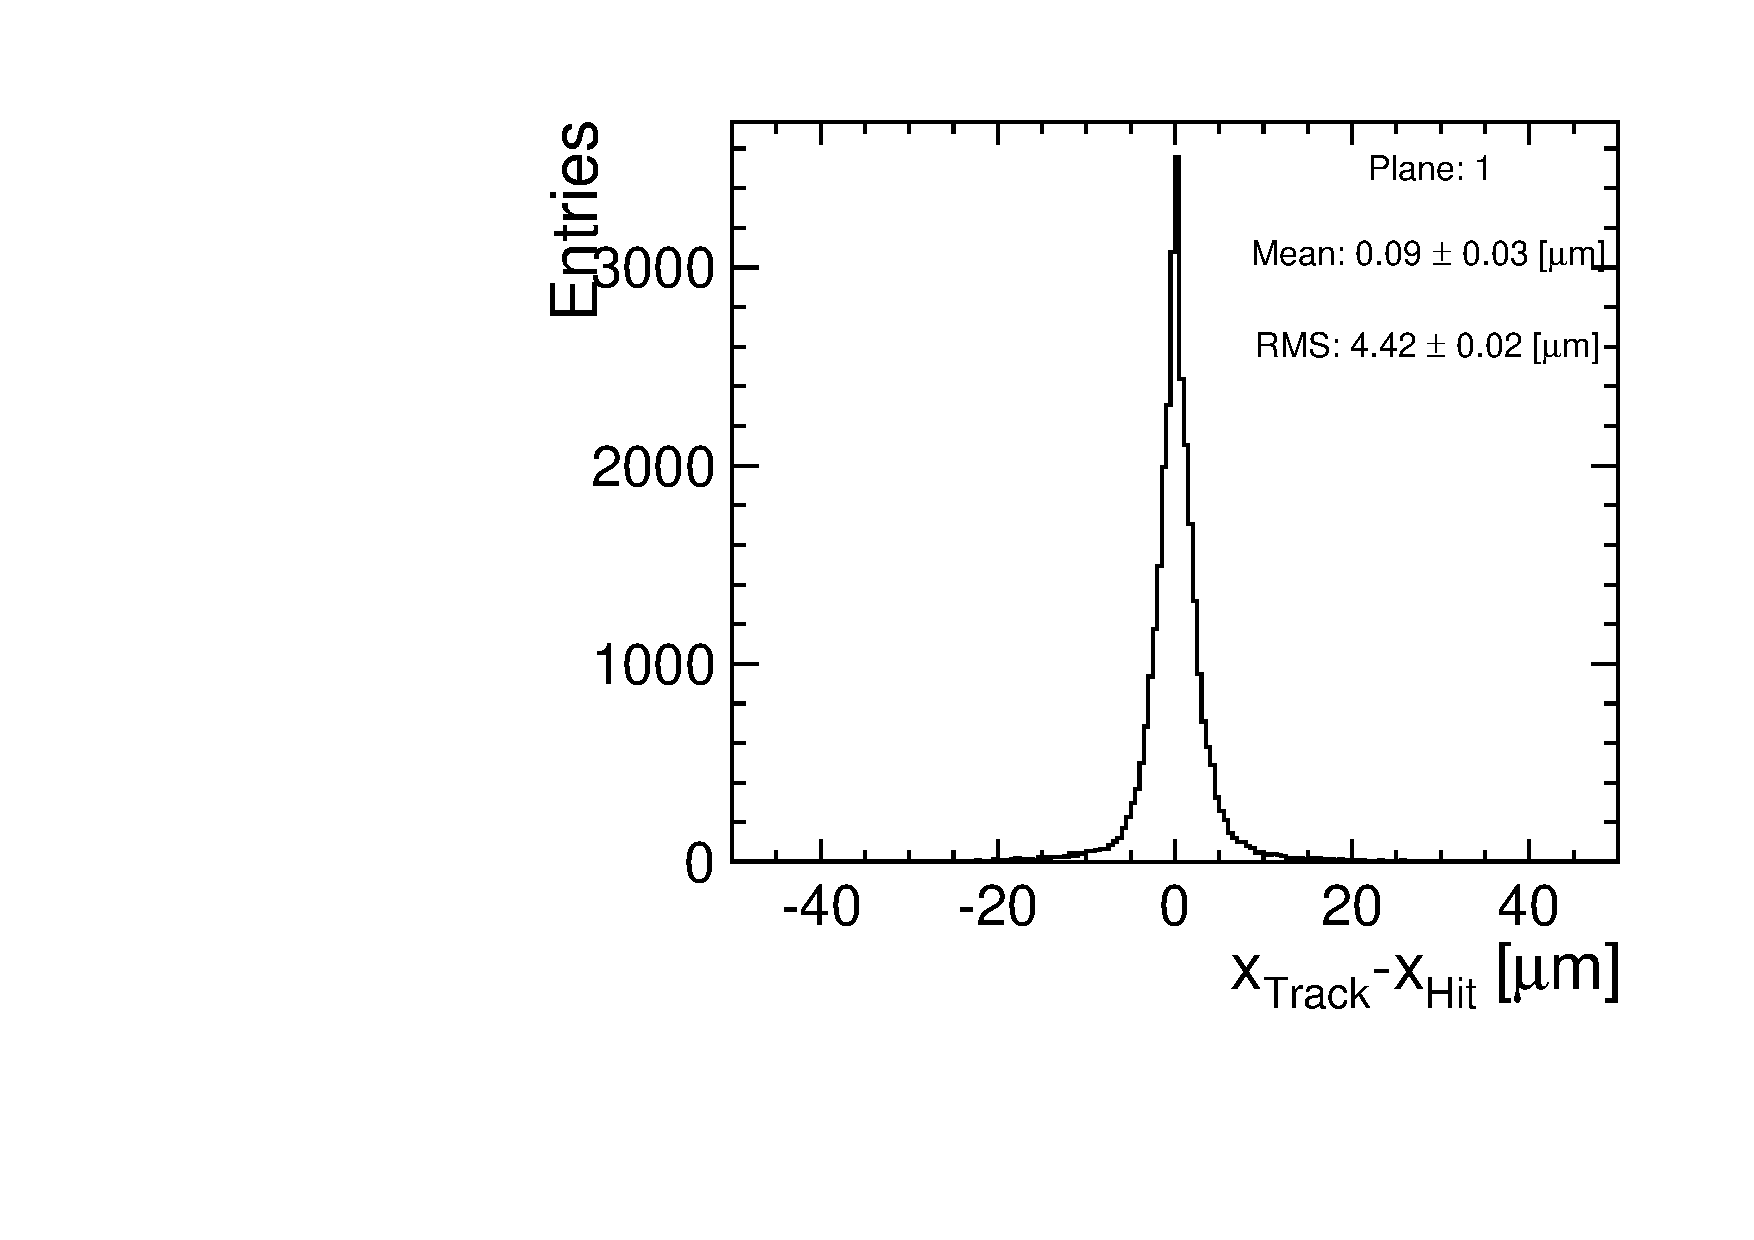
\includegraphics[width=\textwidth]{figures/Telescope/biasedResiduals/BiasedResiduals_run49_PlaneXRMS1.pdf}
    \caption{Telescope plane 1}
  \end{subfigure}\hfill
  \begin{subfigure}[b]{0.3\textwidth}
    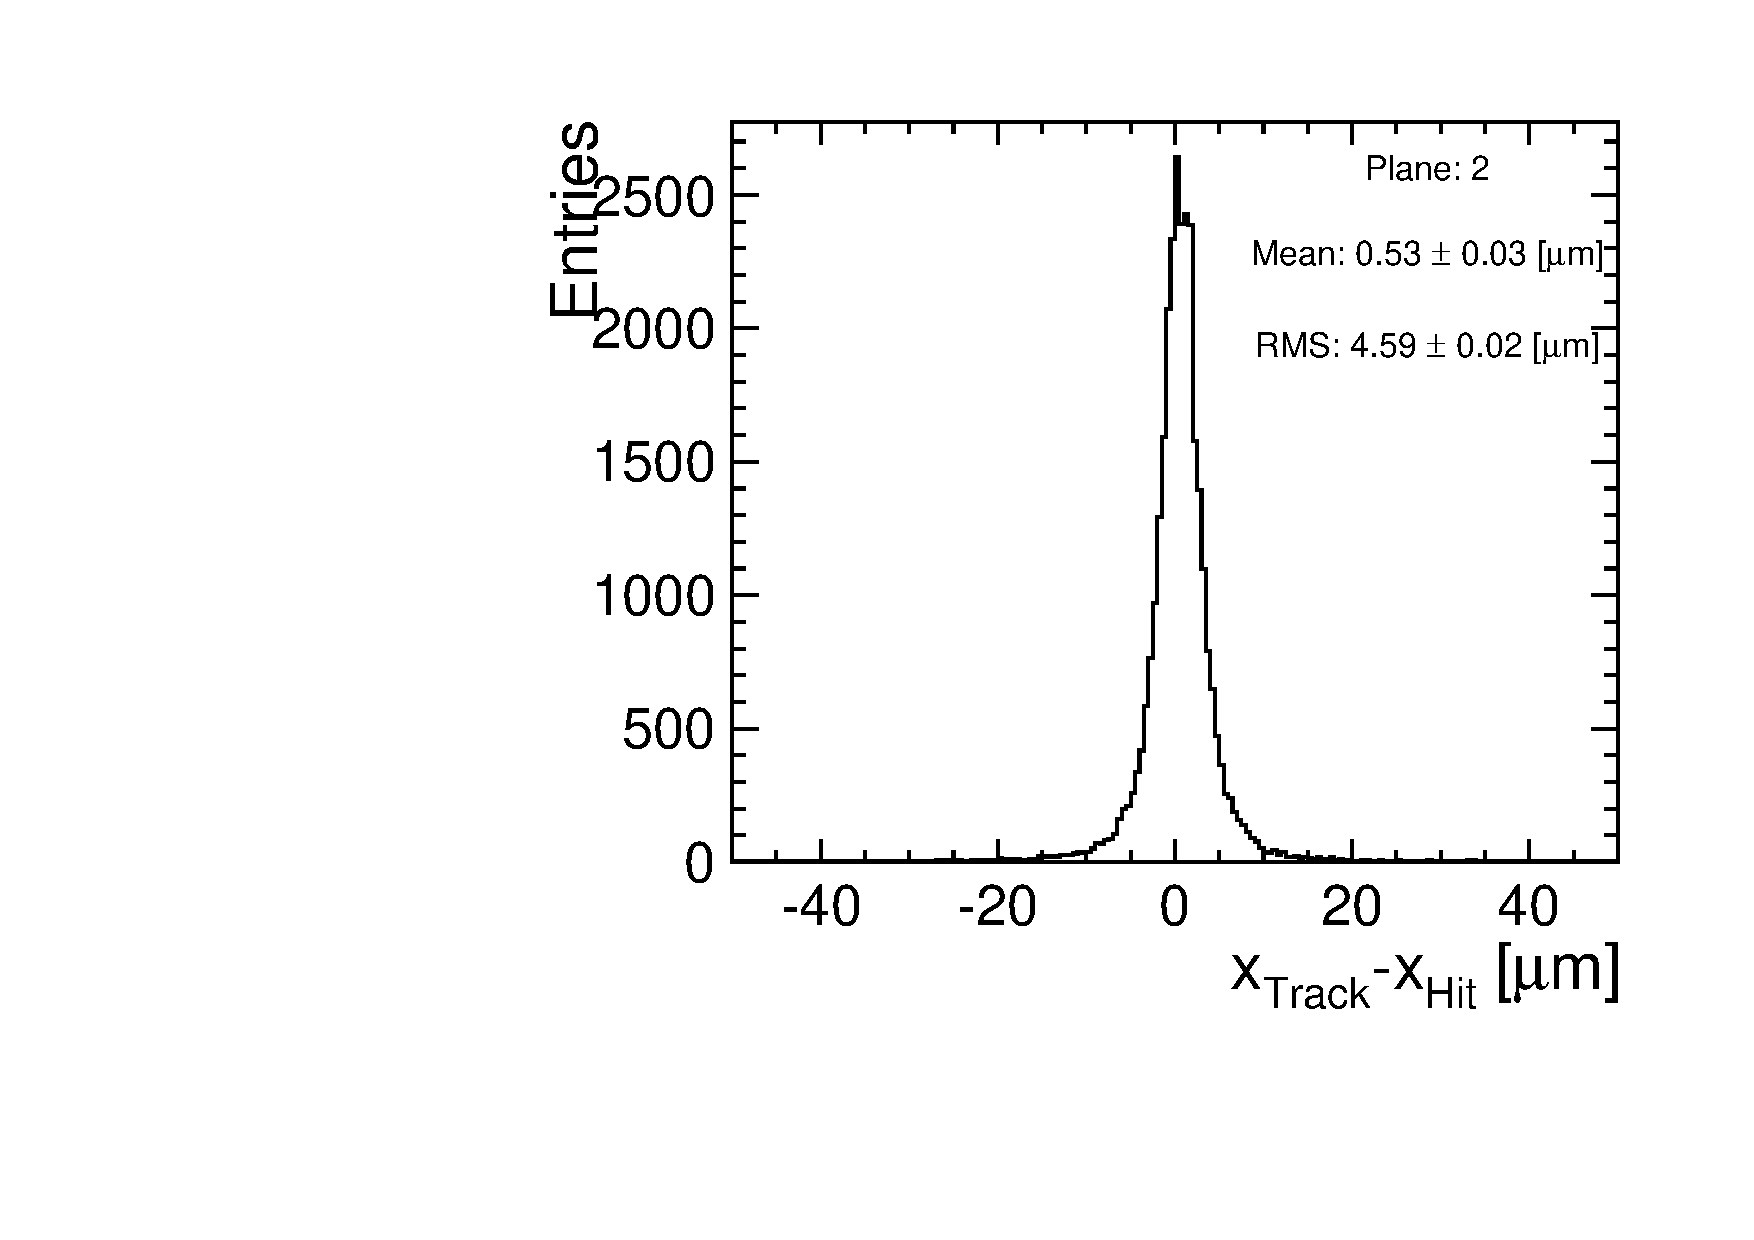
\includegraphics[width=\textwidth]{figures/Telescope/biasedResiduals/BiasedResiduals_run49_PlaneXRMS2.pdf}
    \caption{Telescope plane 2}
  \end{subfigure} \\
  \begin{subfigure}[b]{0.3\textwidth}
    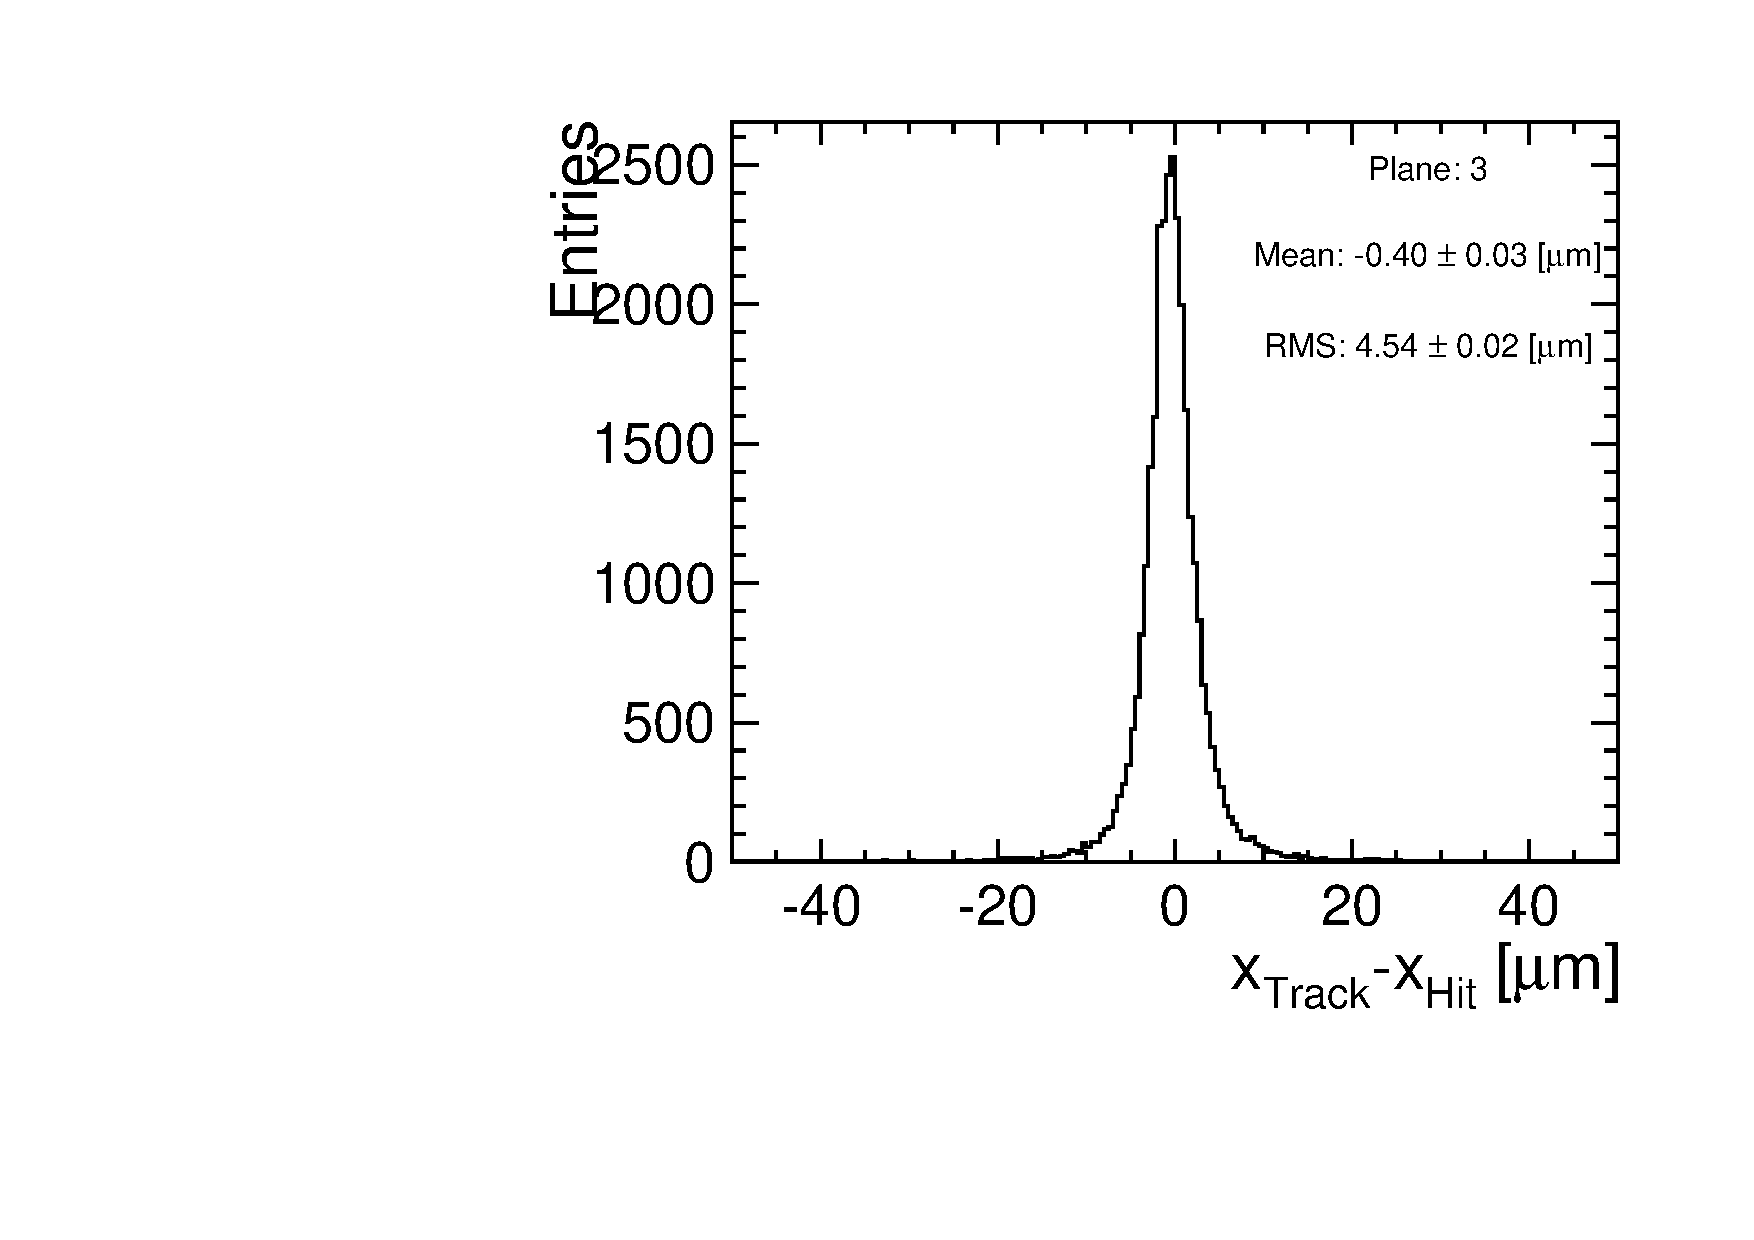
\includegraphics[width=\textwidth]{figures/Telescope/biasedResiduals/BiasedResiduals_run49_PlaneXRMS3.pdf}
    \caption{Telescope plane 3}
  \end{subfigure}\hfill
  \begin{subfigure}[b]{0.3\textwidth}
    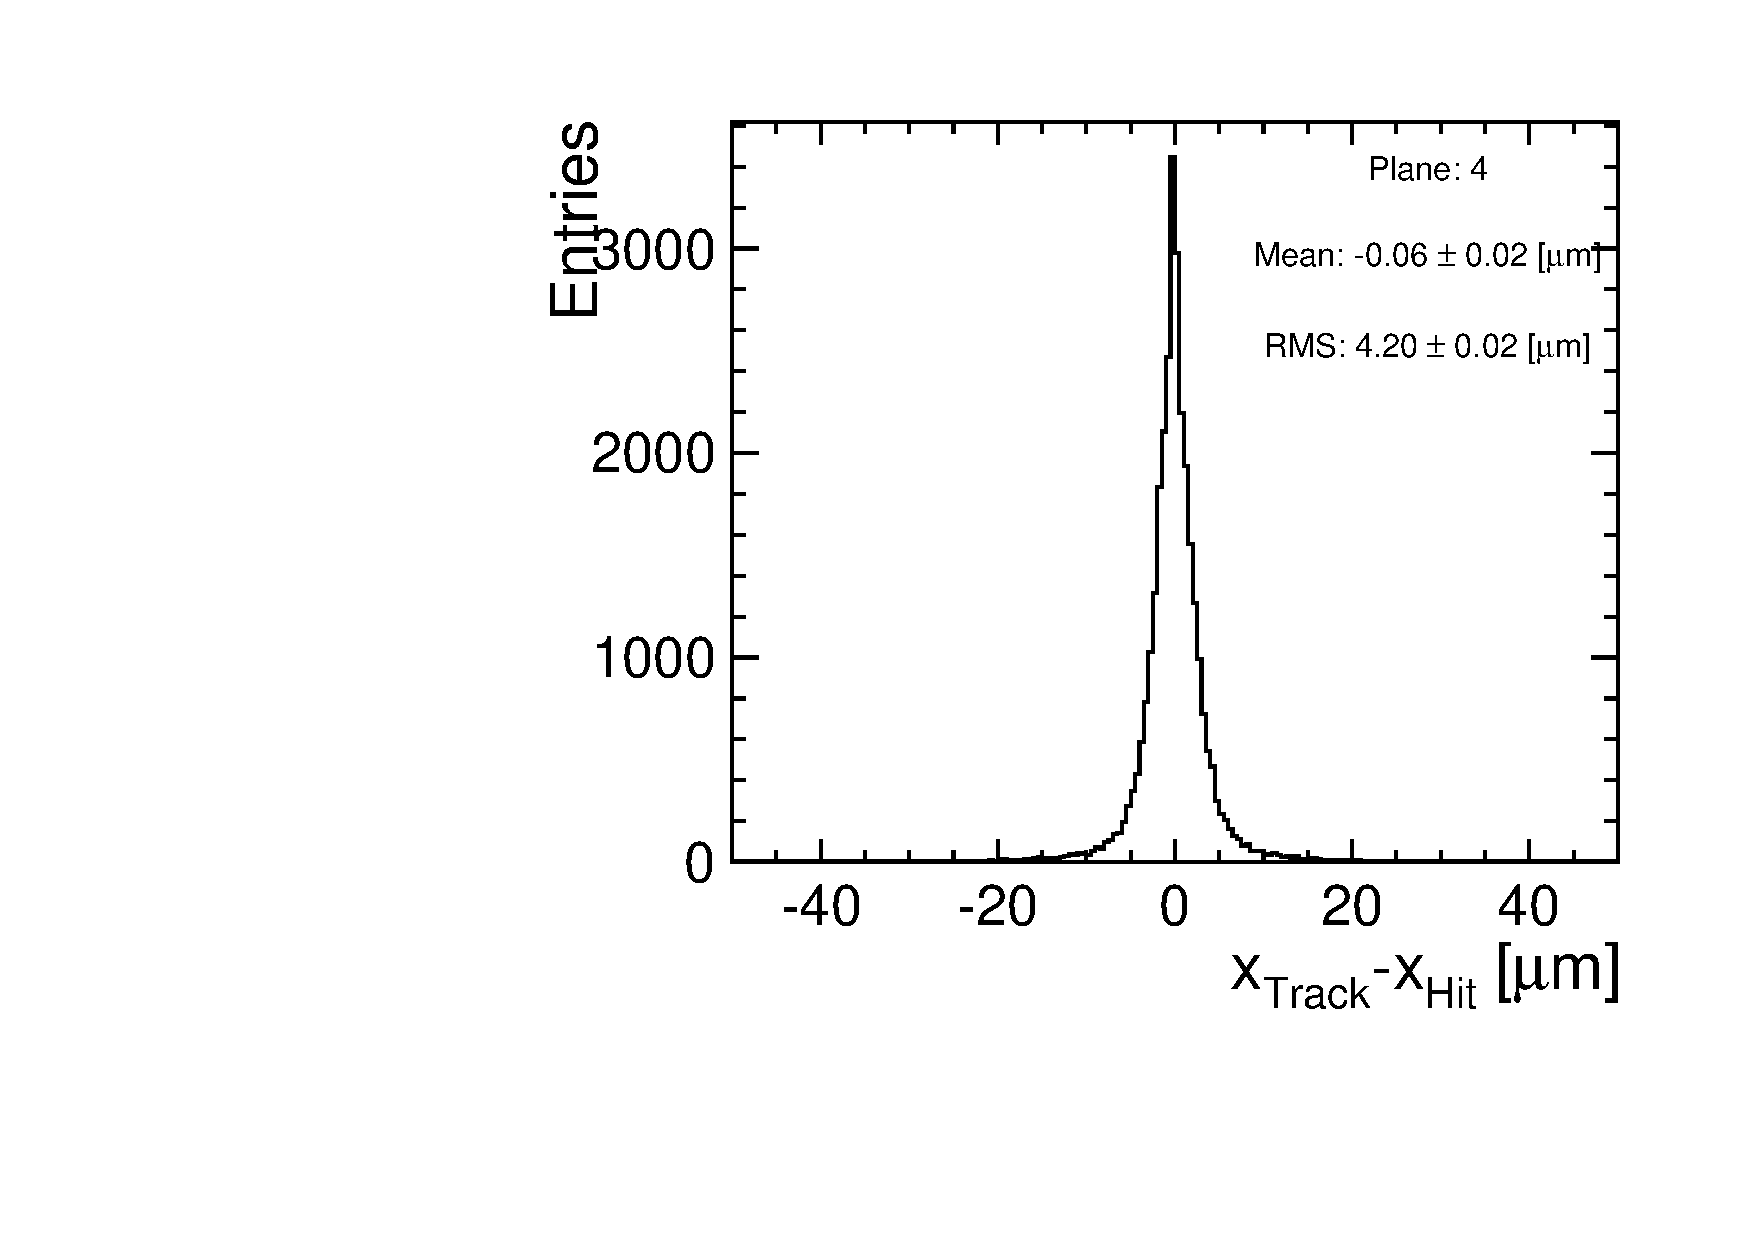
\includegraphics[width=\textwidth]{figures/Telescope/biasedResiduals/BiasedResiduals_run49_PlaneXRMS4.pdf}
    \caption{Telescope plane 4}
  \end{subfigure}\hfill
  \begin{subfigure}[b]{0.3\textwidth}
    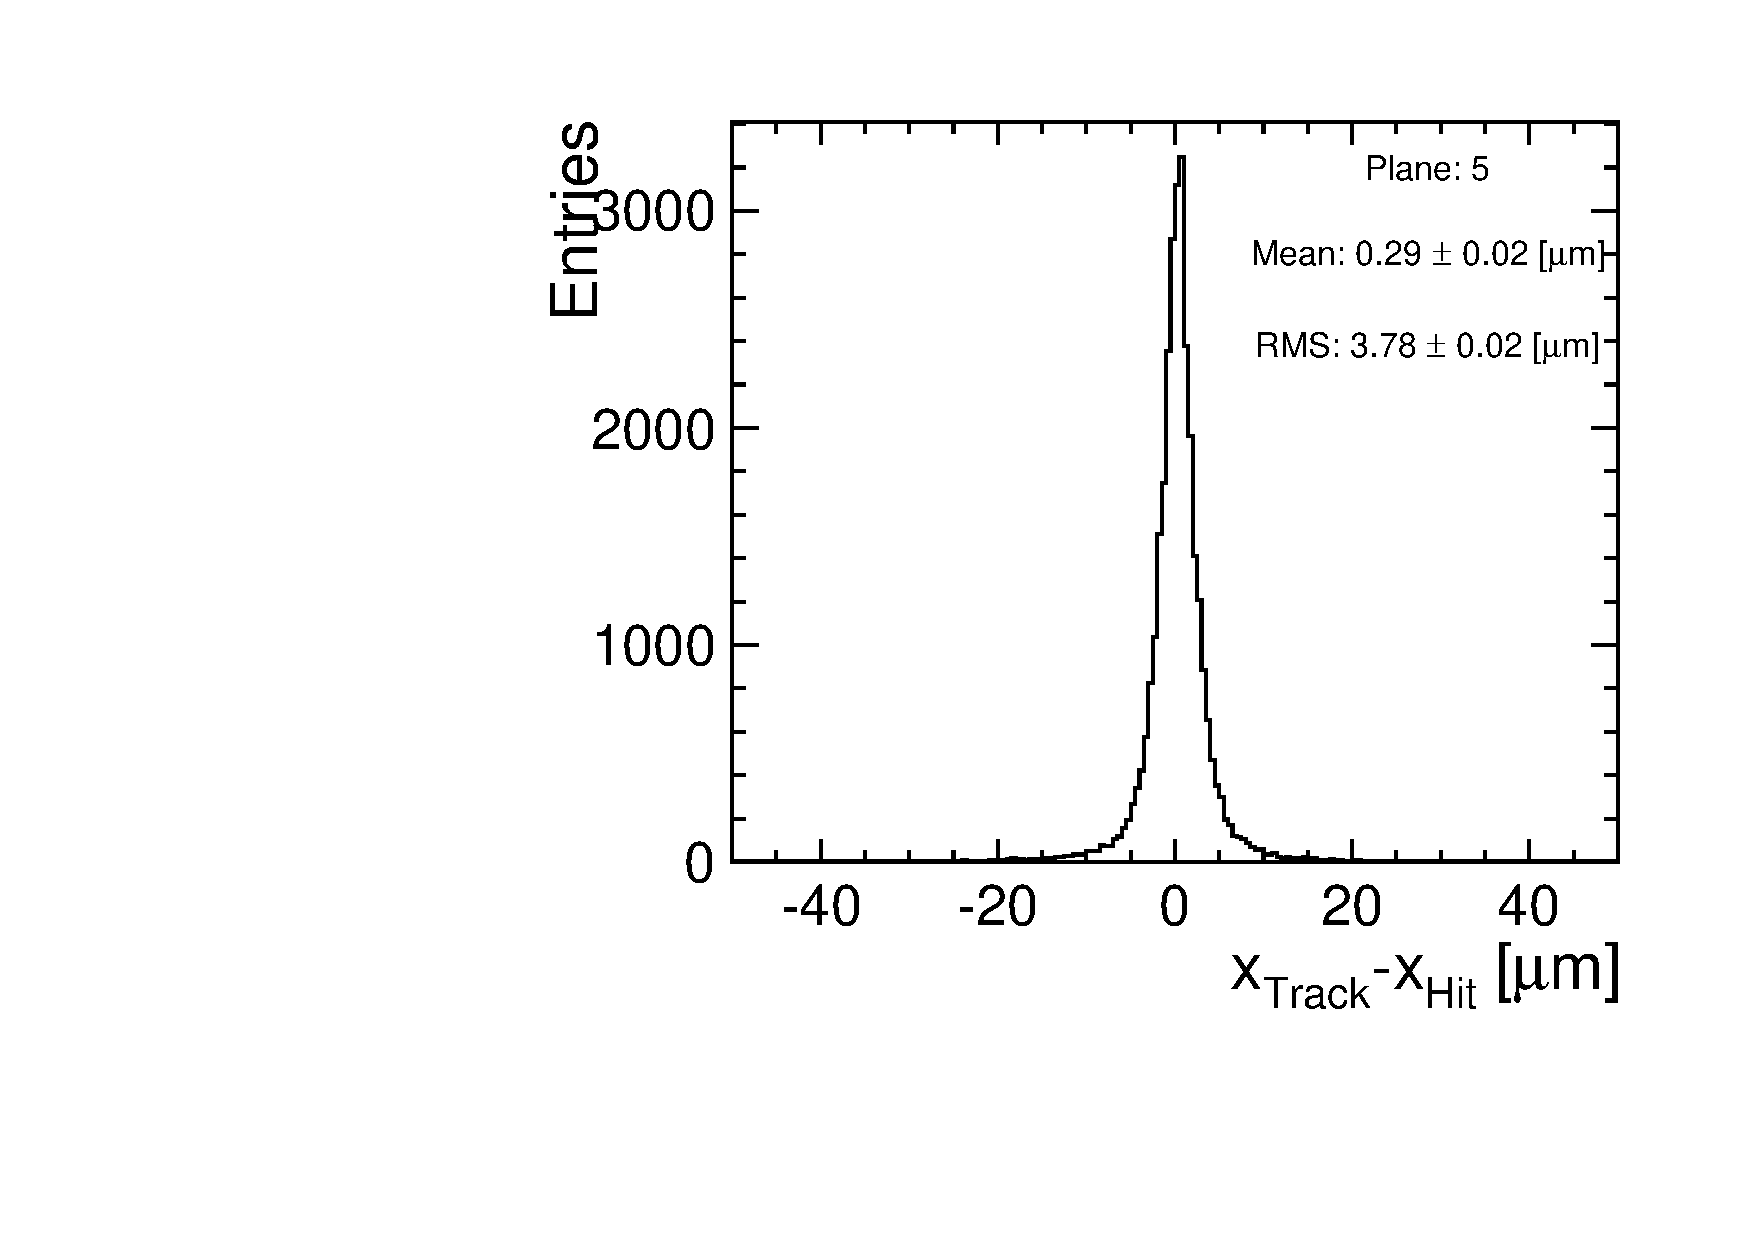
\includegraphics[width=\textwidth]{figures/Telescope/biasedResiduals/BiasedResiduals_run49_PlaneXRMS5.pdf}
    \caption{Telescope plane 5}
  \end{subfigure}
  \caption{Biased residual distribution in x-direction obtained in
    AllPix simulations for each telescope plane. The RMS of the
    residual is also shown.}
  \label{fig:telescope_biasedResiduals_simu_X}
\end{figure}

\begin{figure}[htbp] \centering
  \begin{subfigure}[b]{0.3\textwidth}
    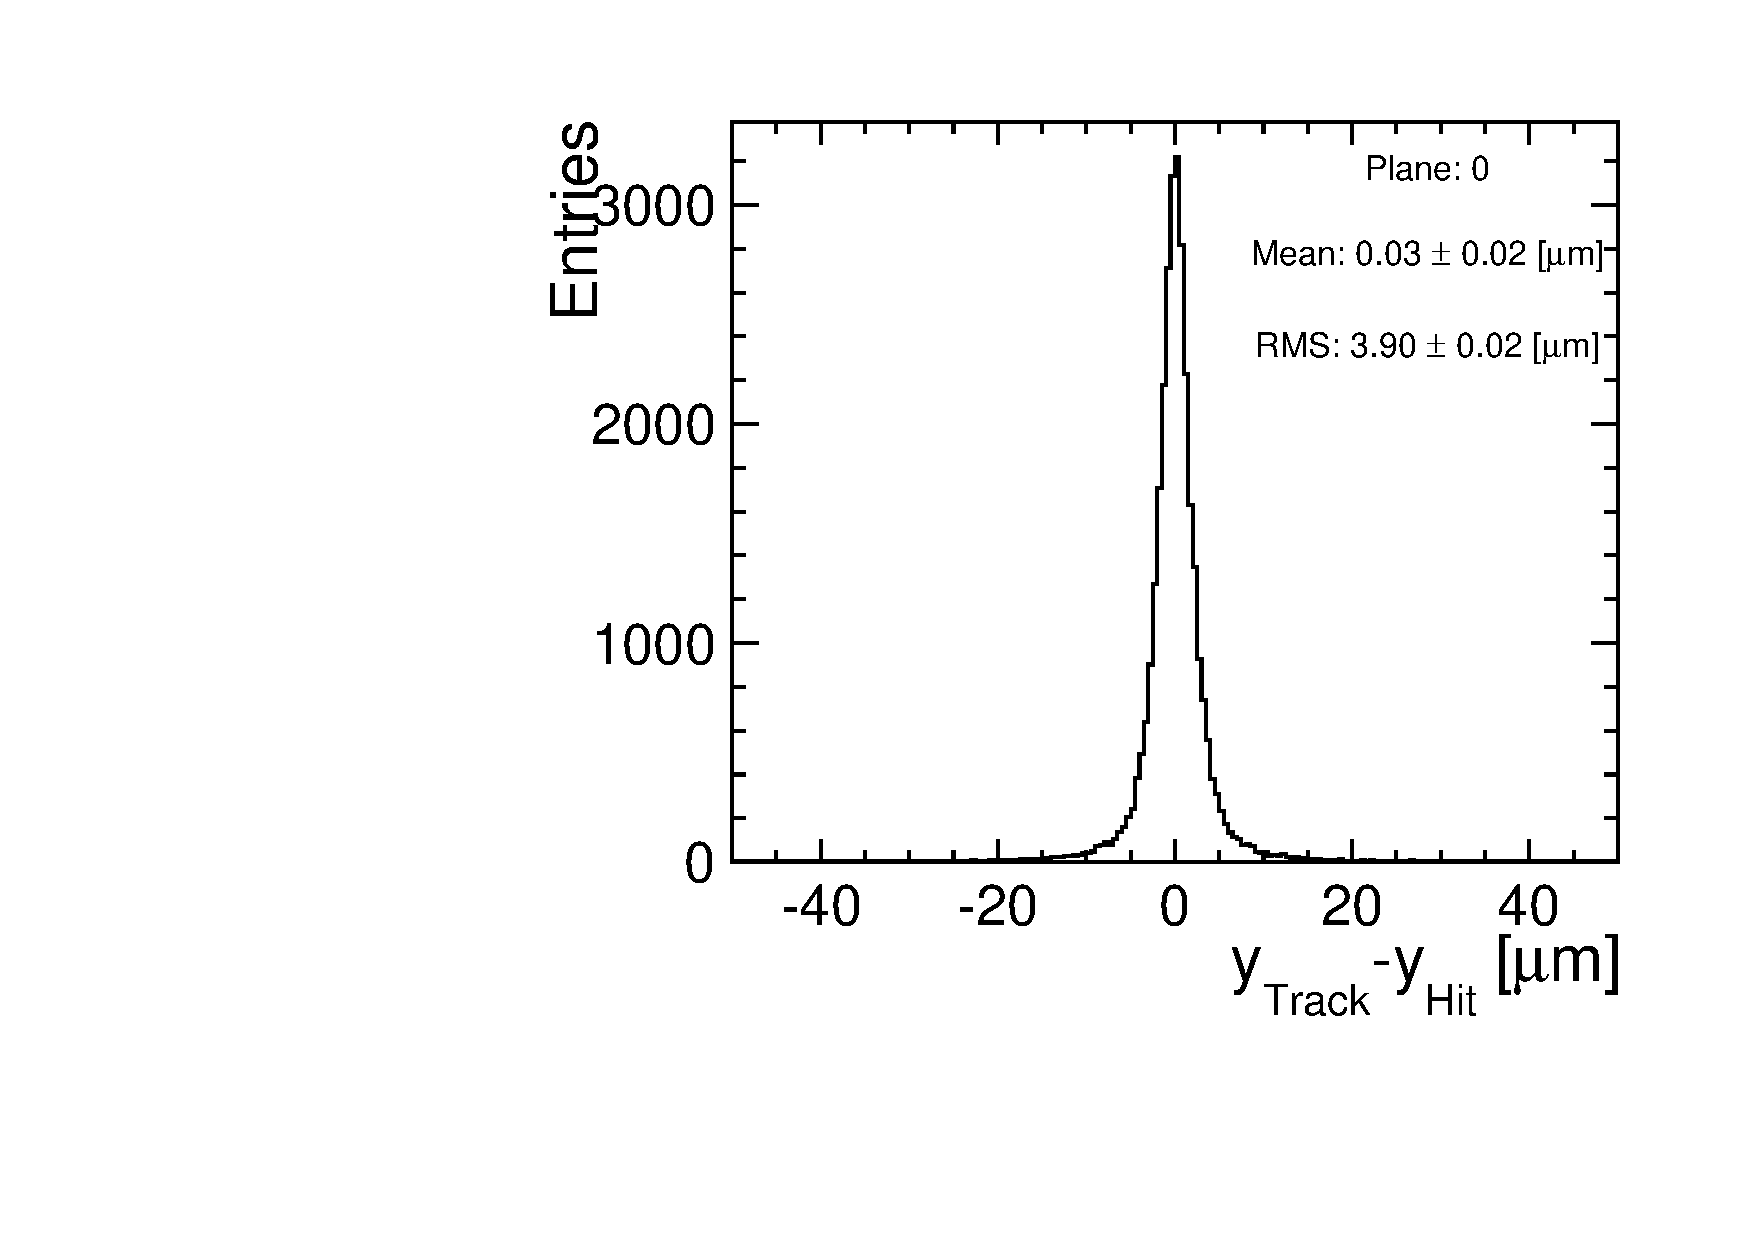
\includegraphics[width=\textwidth]{figures/Telescope/biasedResiduals/BiasedResiduals_run49_PlaneYRMS0.pdf}
    \caption{Telescope plane 0}
  \end{subfigure}\hfill
  \begin{subfigure}[b]{0.3\textwidth}
    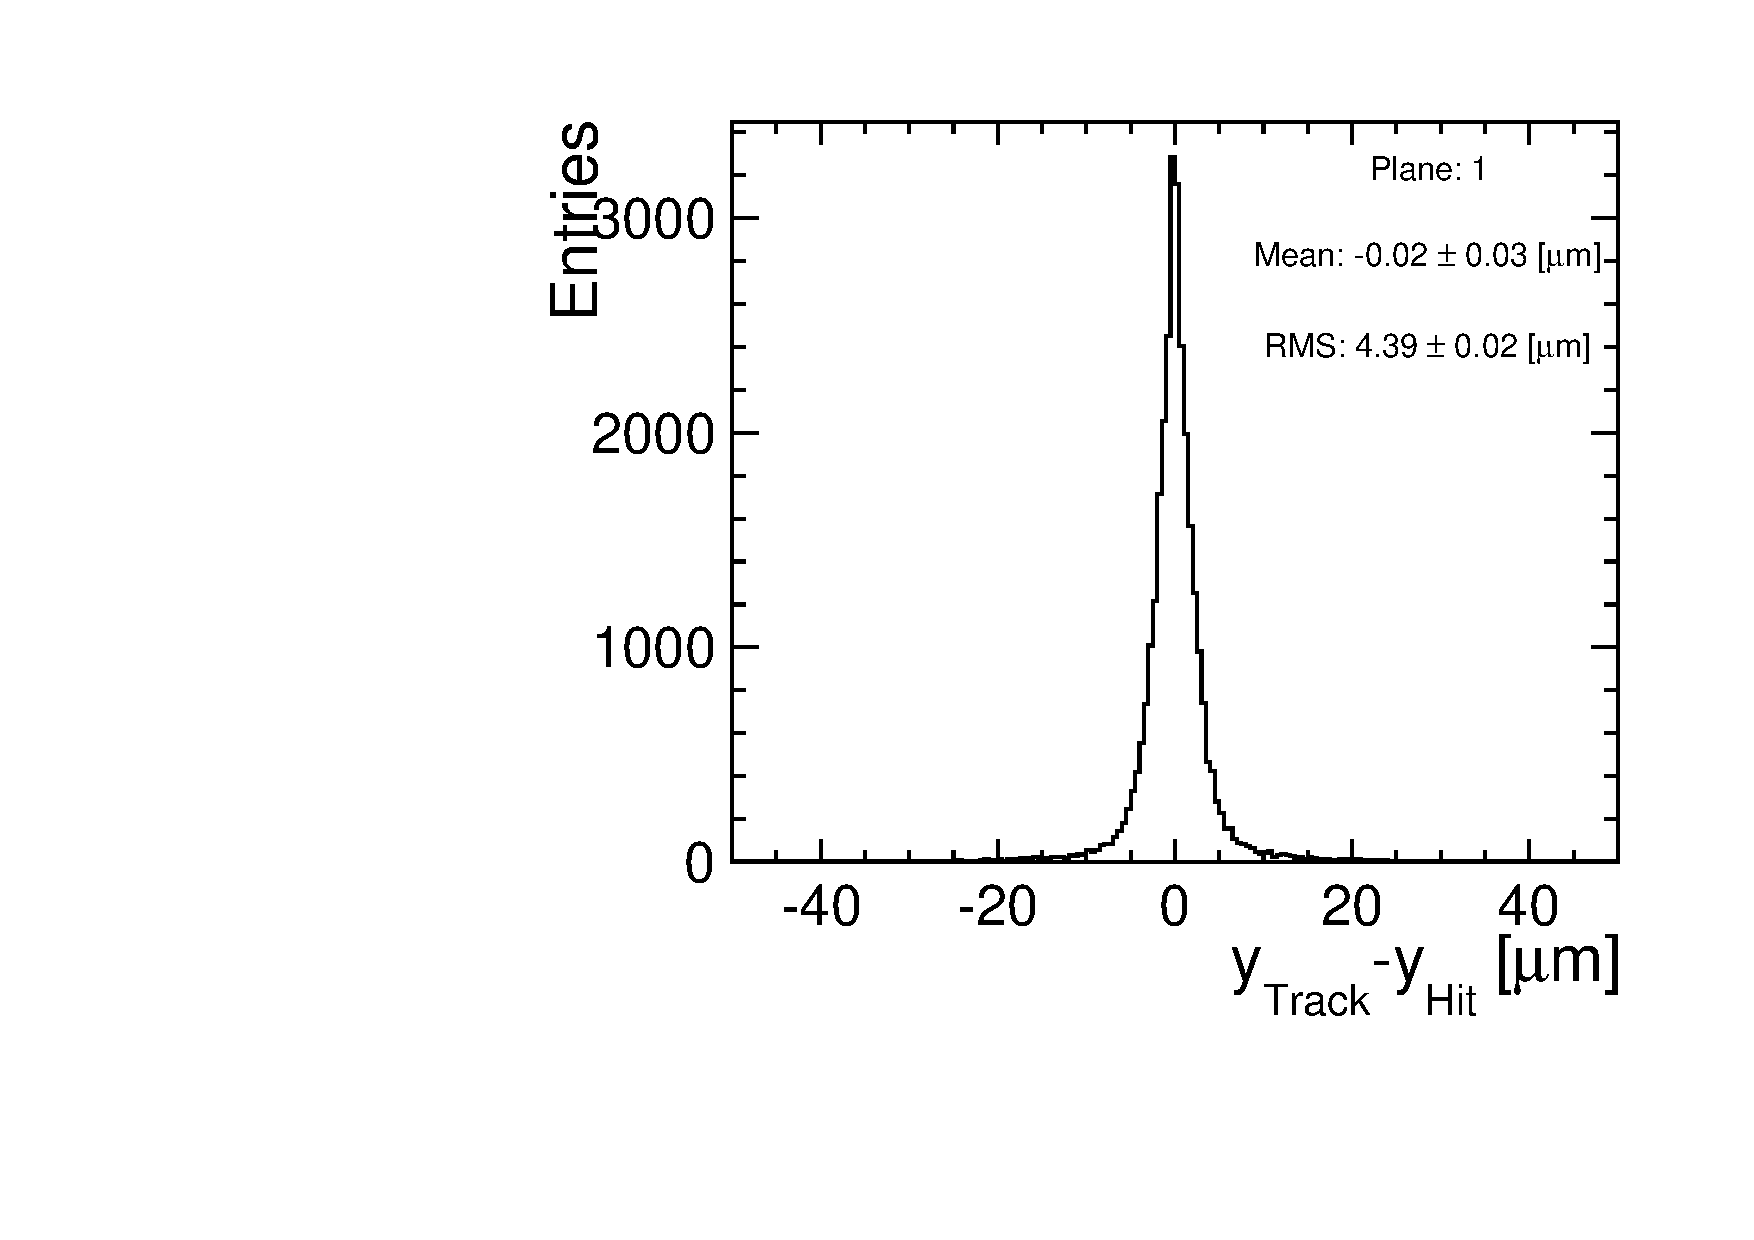
\includegraphics[width=\textwidth]{figures/Telescope/biasedResiduals/BiasedResiduals_run49_PlaneYRMS1.pdf}
    \caption{Telescope plane 1}
  \end{subfigure}\hfill
  \begin{subfigure}[b]{0.3\textwidth}
    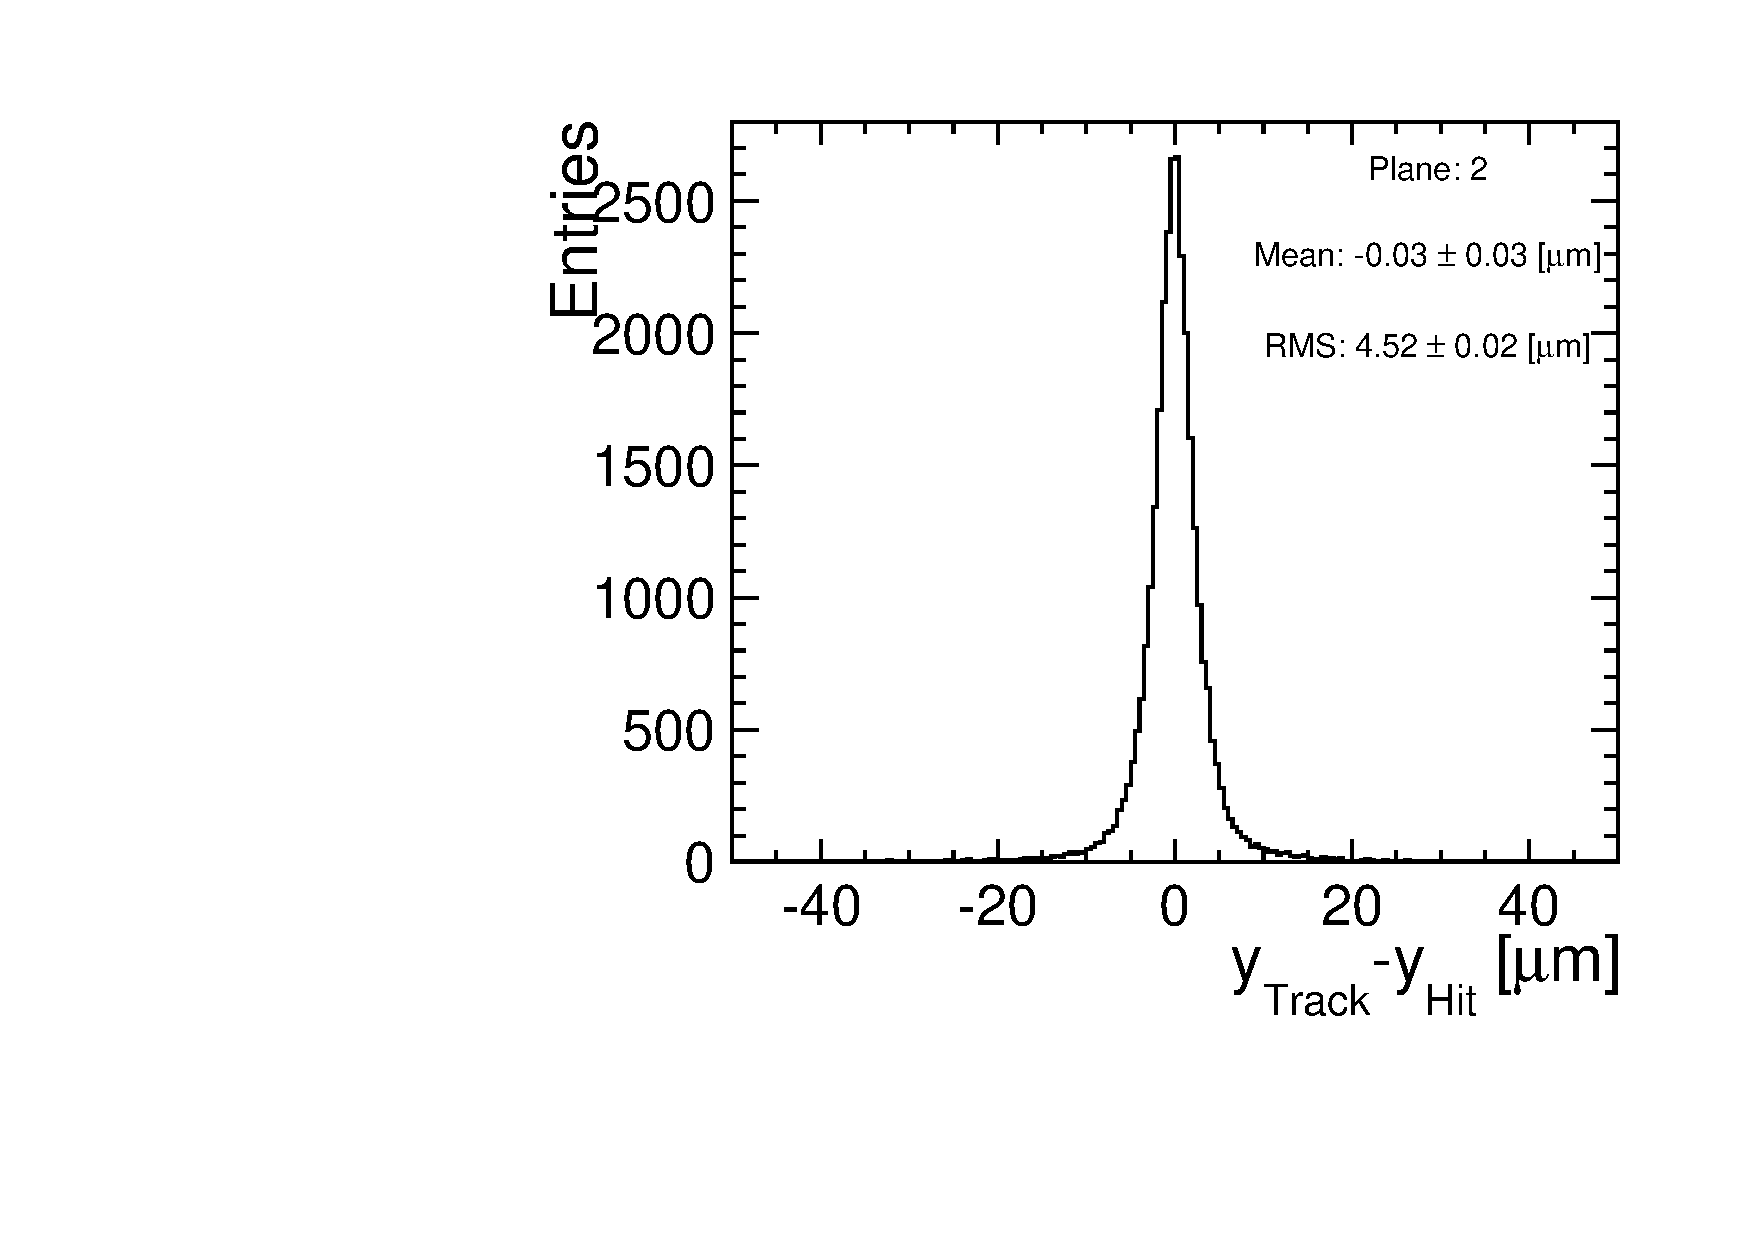
\includegraphics[width=\textwidth]{figures/Telescope/biasedResiduals/BiasedResiduals_run49_PlaneYRMS2.pdf}
    \caption{Telescope plane 2}
  \end{subfigure} \\
  \begin{subfigure}[b]{0.3\textwidth}
    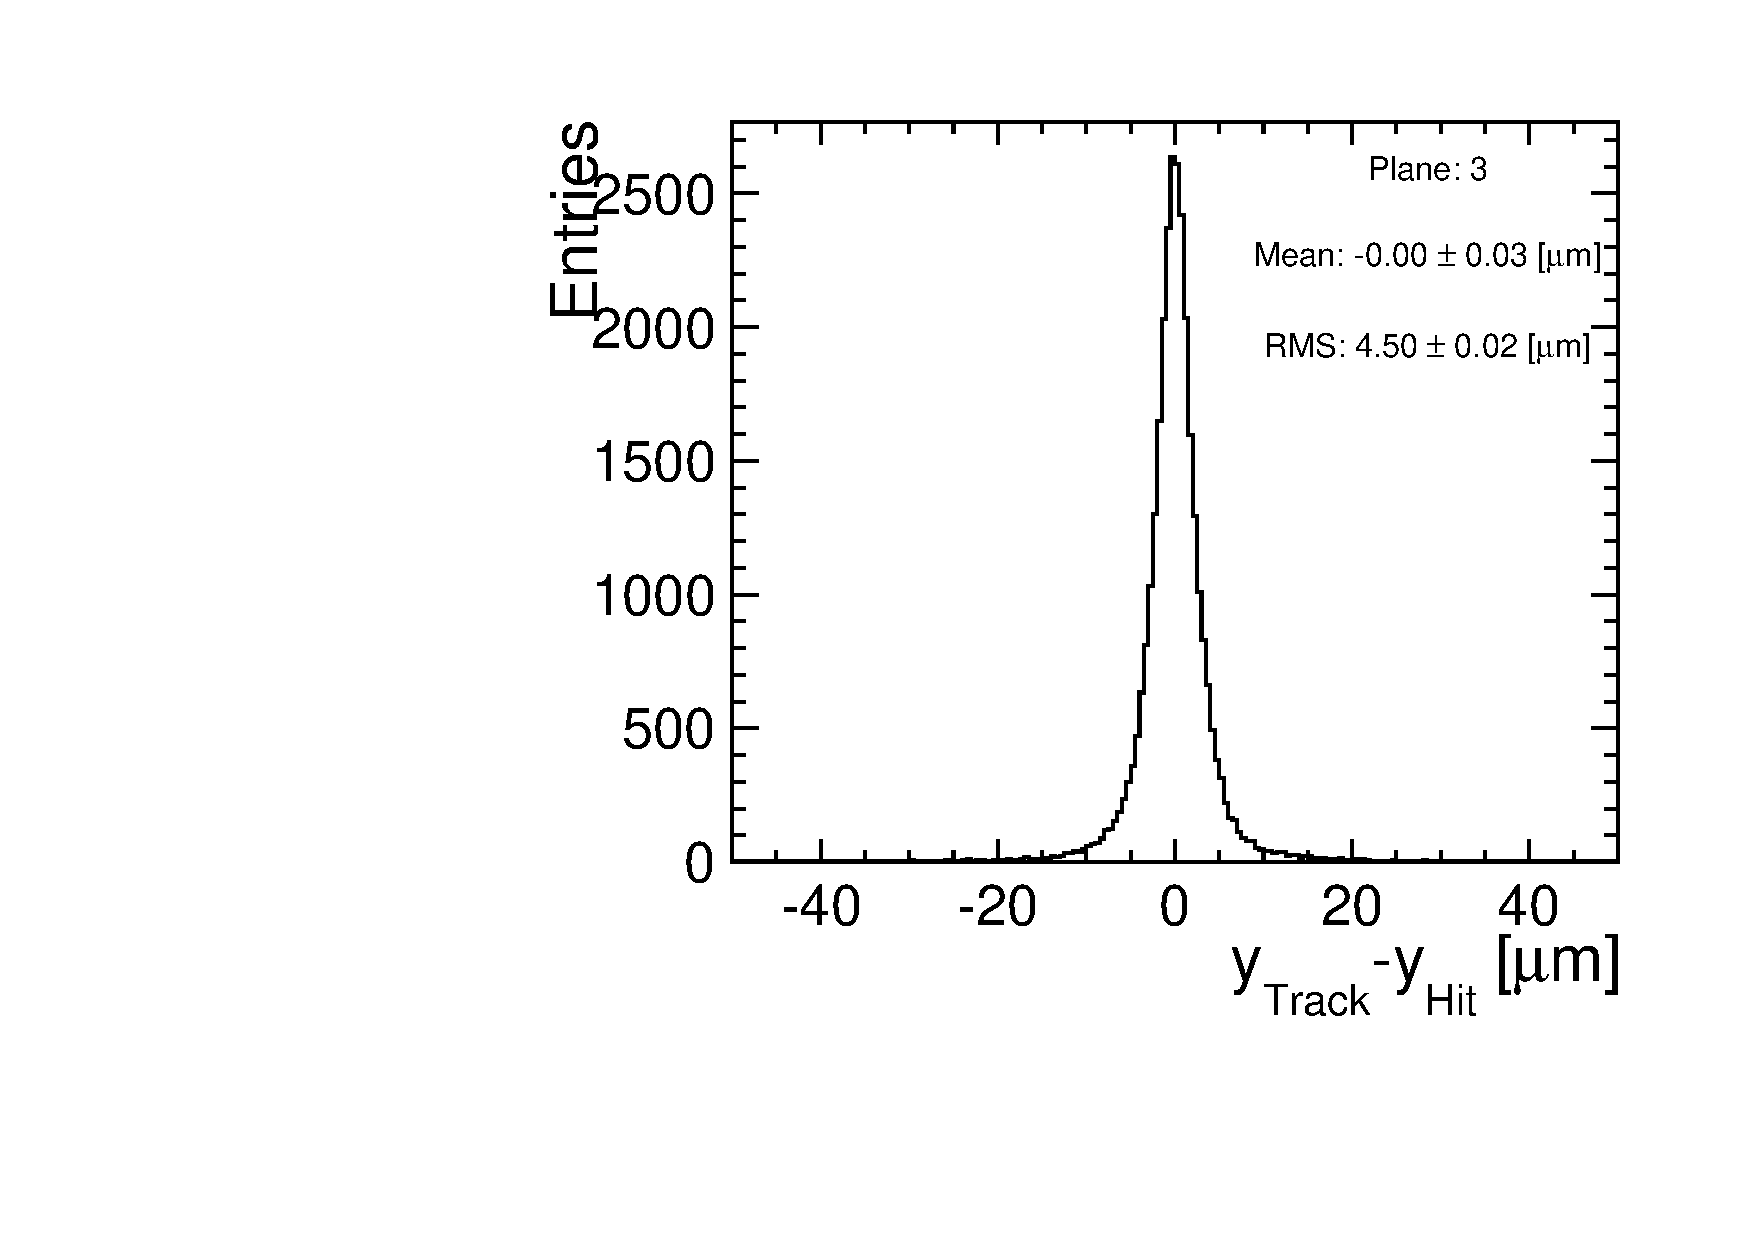
\includegraphics[width=\textwidth]{figures/Telescope/biasedResiduals/BiasedResiduals_run49_PlaneYRMS3.pdf}
    \caption{Telescope plane 3}
  \end{subfigure}\hfill
  \begin{subfigure}[b]{0.3\textwidth}
    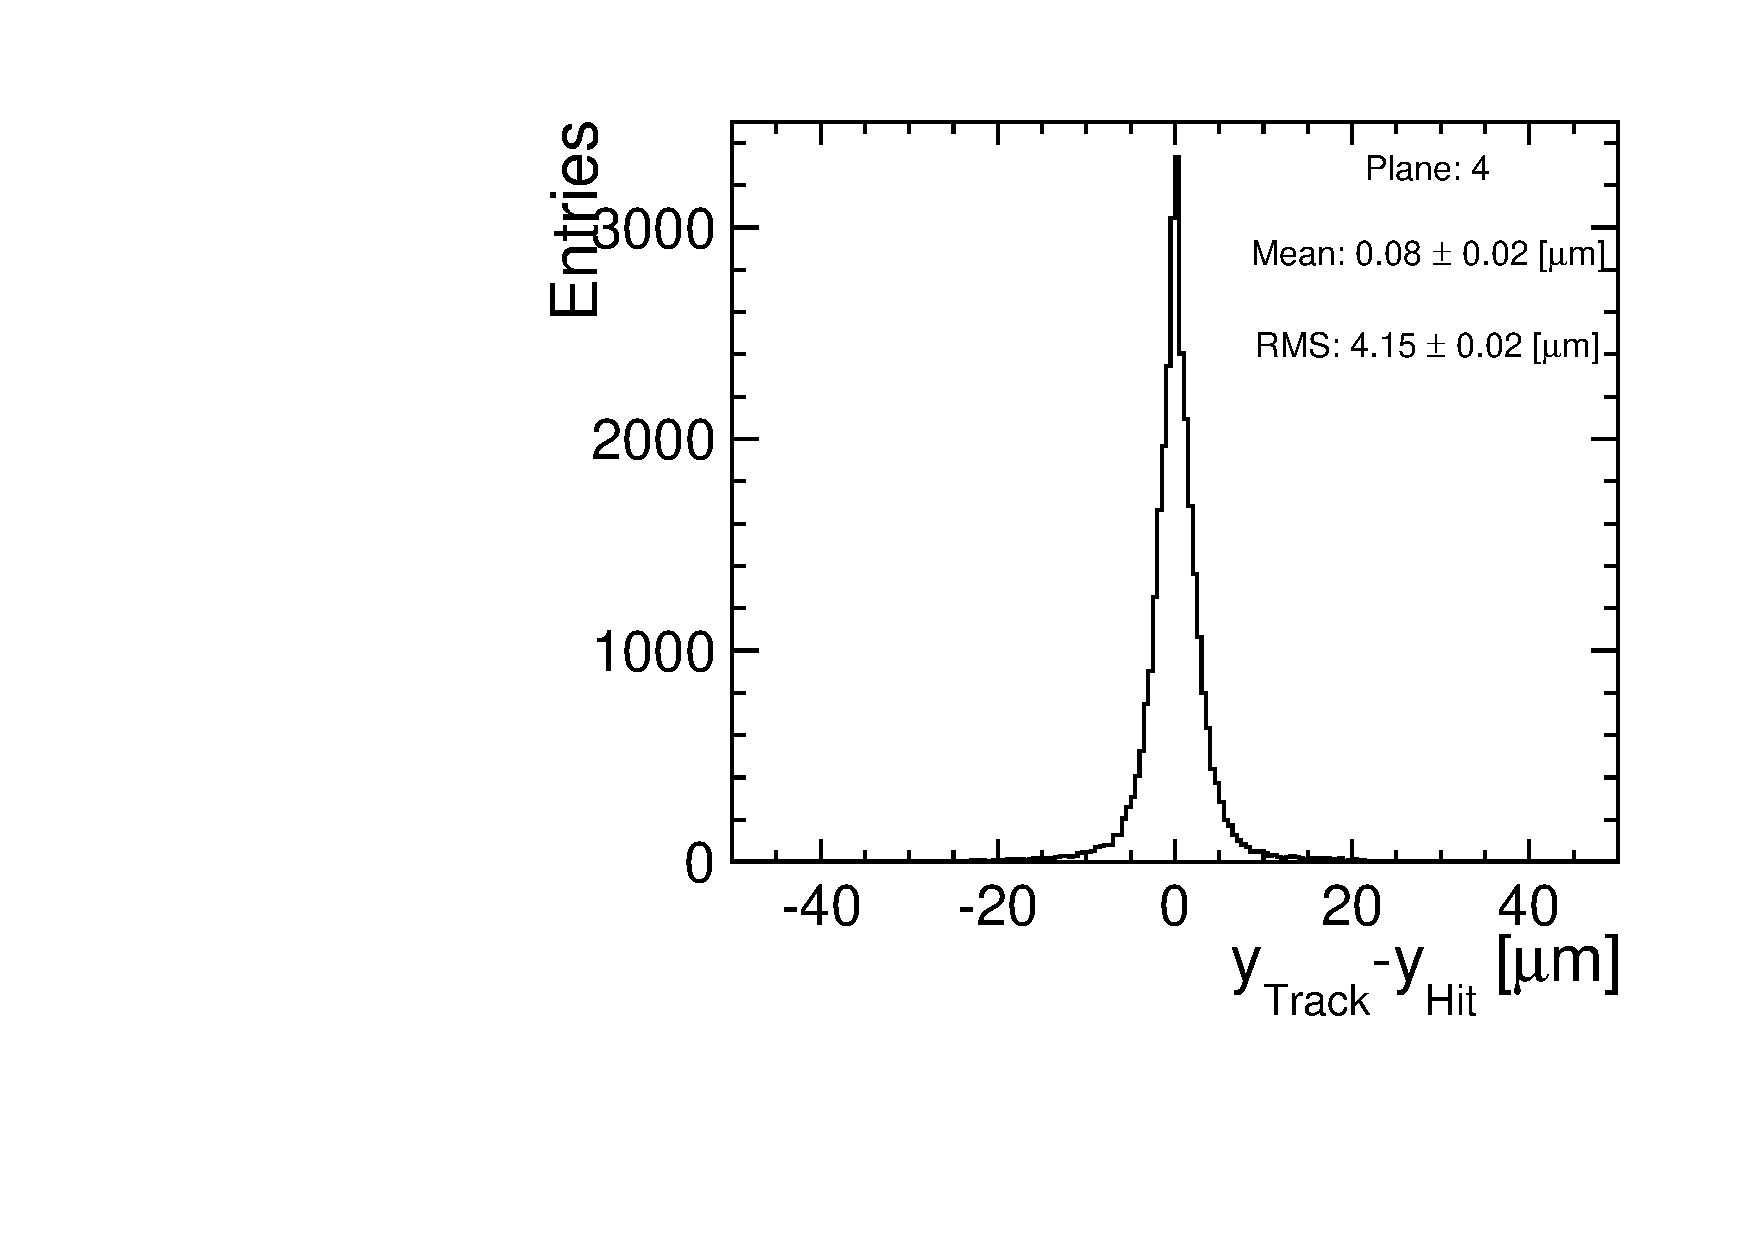
\includegraphics[width=\textwidth]{figures/Telescope/biasedResiduals/BiasedResiduals_run49_PlaneYRMS4.pdf}
    \caption{Telescope plane 4}
  \end{subfigure}\hfill
  \begin{subfigure}[b]{0.3\textwidth}
    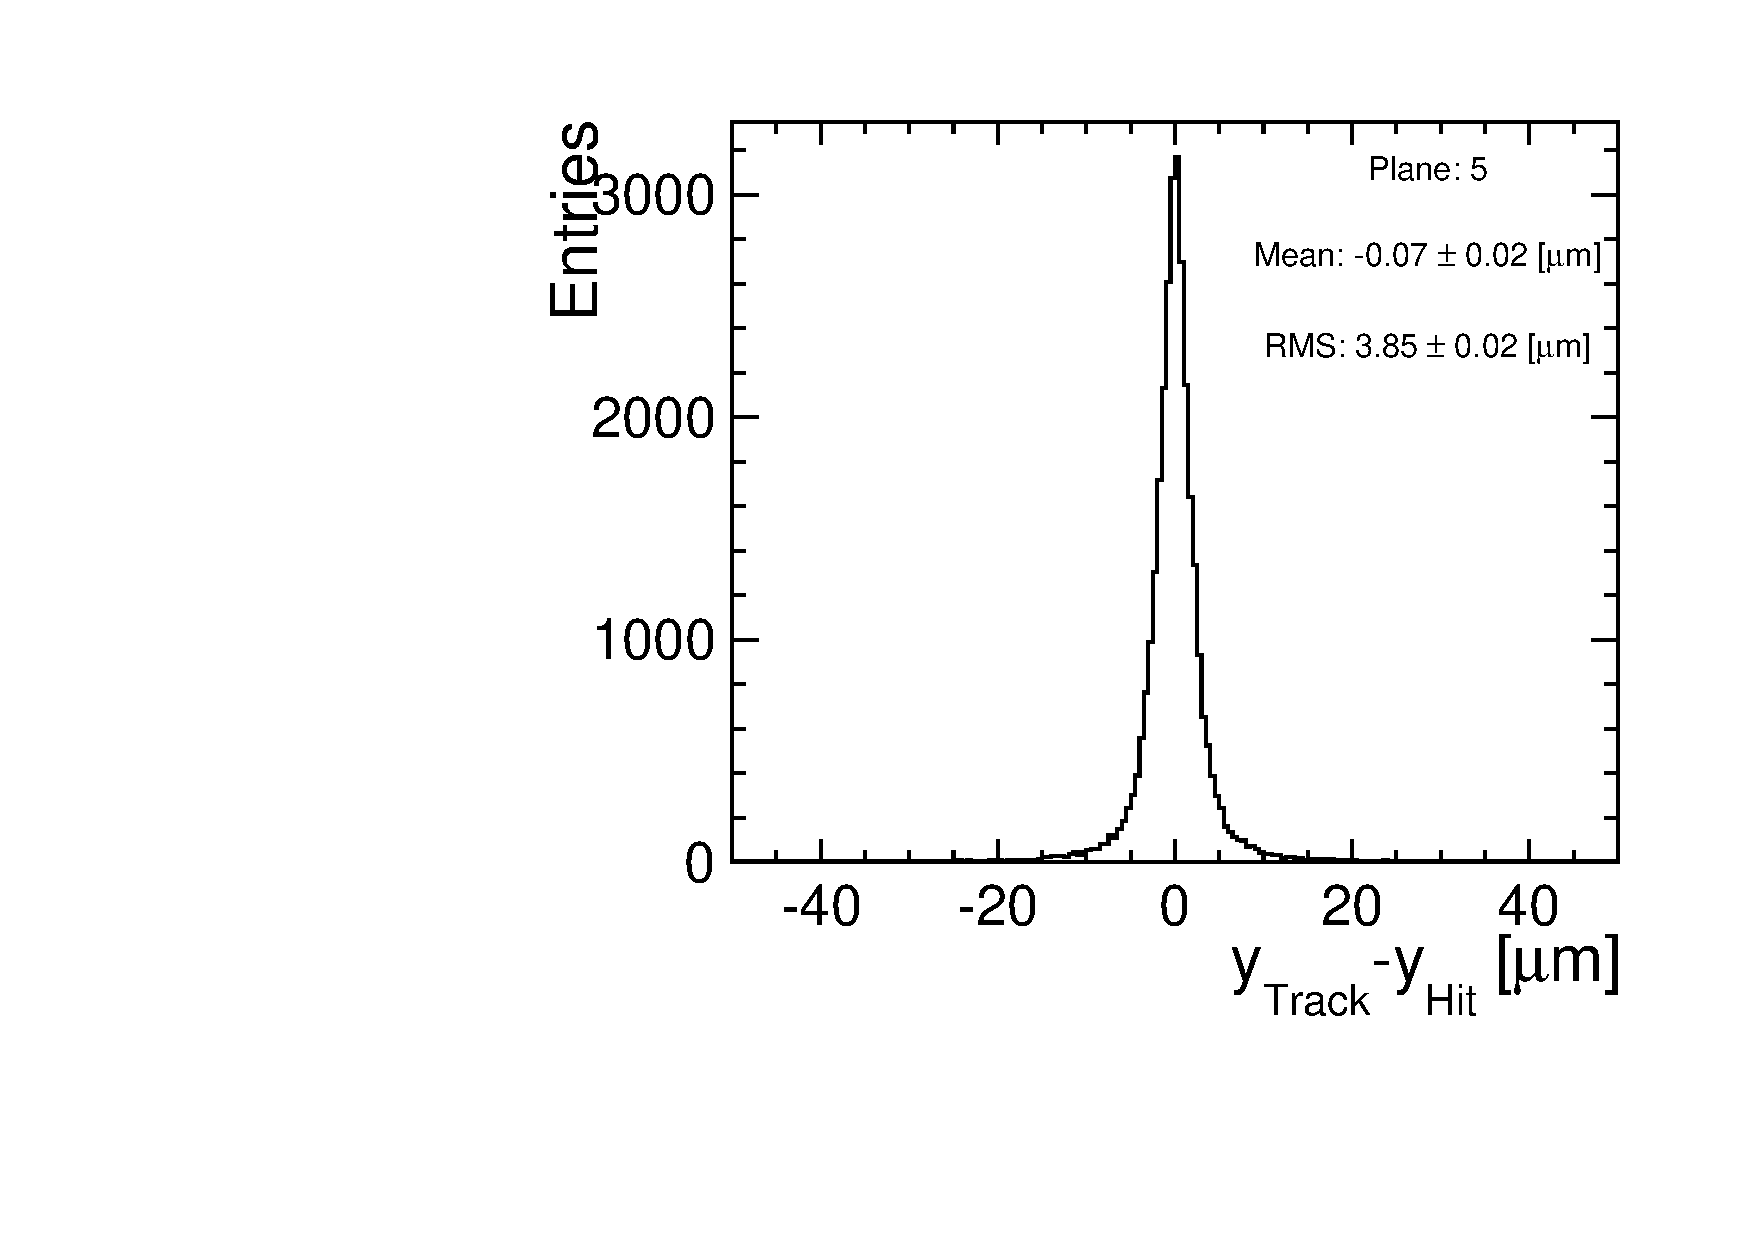
\includegraphics[width=\textwidth]{figures/Telescope/biasedResiduals/BiasedResiduals_run49_PlaneYRMS5.pdf}
    \caption{Telescope plane 5}
  \end{subfigure}
  \caption{Biased residual distribution in y-direction obtained in
    AllPix simulations for each telescope plane. The RMS of the
    residual is also shown.}
  \label{fig:telescope_biasedResiduals_simu_Y}
\end{figure}
